\documentclass[12pt]{article}

\usepackage{graphicx} % This lets you include figures
\usepackage{hyperref} % This lets you make links to web locations
\graphicspath{ {./images/} }

\usepackage[a4paper,text={18cm, 24.2cm}, left=1.8cm, top=1.8cm]{geometry}

\usepackage[rightcaption]{sidecap}
\usepackage{subcaption}
\usepackage{wrapfig}

\usepackage[czech]{babel}
\usepackage[utf8]{inputenc}

\usepackage{float}

\usepackage{imakeidx}

\makeindex


\title{C-Real Manual}
\author{}
\date{\today}

\begin{document}
\maketitle{}

\tableofcontents

\clearpage
\newpage

\section{Systémové požadavky}

\begin{itemize}
    \item Operační systém:
    \begin{itemize}
        \item Windows 11
        \item Ubuntu 24.04 LTS nebo novější
    \end{itemize}
    \item Minimálně 200\,MB volného místa
    \item Přístup k internetu pouze při stažení balíčku
    \item Pro manuální instalaci:
    \begin{itemize}
        \item \href{https://docs.flutter.dev/install}{Flutter}
        \item Git
        \item GNU make
        \item \href{https://aka.ms/vs/stable/vs_BuildTools.exe}{Balíček: Desktop developement with C++}
        \item \href{}{CMake (pro Ubuntu)}
        \item \href{}{Ninja-build (pro Ubuntu)}
        \item \href{}{Clangd (pro Ubuntu)}
        \item \href{}{Libgtk-3-dev (pro Ubuntu)}
        
    \end{itemize}
\end{itemize}

\vspace{1.0cm}

\section{Instalace/odinstalace pomocí instalátoru}

\subsection{Windows}

\subsubsection{Postup instalace:}
\begin{enumerate}
    \item Stáhněte soubor \textbf{C-Real-Setup-Windows.exe}.
    \item Spusťte instalační soubor dvojklikem.
    \item Pokude se objeví bezpečnostní upozornení systému Windows, potvrďte spuštení.
    \item V instalačním průvodci klikněte na \textbf{Next}
    \item Vyberte cílovou zložku instalace.
    \item Zvolte zda se má vytvořit:
    \begin{itemize}
        \item zástupce na ploše,
        \item zástupce v nabídce start.
    \end{itemize}
    \item Dokončete tlačitkem \textbf{Install}
    \item Po dokončení lze program ihned spusťit volbou \textbf{Lauch C-Real}
\end{enumerate}

\emph{Instalátor provede tyto změny:}
\begin{itemize}
    \item zkopíruje soubory programu do instlační složky,
    \item vytvoři zástupce v nabídce Start,
    \item volitelně vytvoři ikonu na ploše,
    \item zaregistruje odinstalátor do systému.
\end{itemize}

\subsubsection{Postup odinstalace:}
Program lze odinstalovat jedným z následujících způsobů.\newline

\noindent Možnost A:
\begin{enumerate}
    \item Otevřete \textbf{nastavení $\rightarrow$ aplikace},
    \item V Seznamu vyhledejte \textbf{C-Real},
    \item Klikněte na \textbf{Odistalovat}.
\end{enumerate}

\noindent Možnost B:
\begin{enumerate}
    \item Otevřete \textbf{instalační složku programu},
    \item Dvojklikem spusťte soubor \textbf{unins000.exe},
    \item Potvrďte odinstalaci.
\end{enumerate}

\noindent Odinstalátor provede následovné:
\begin{itemize}
    \item odstraní soubory programu,
    \item odstraní zástupce vytvořené instalátorem,
    \item odebere položku ze seznamu naistalovaných aplikací.
\end{itemize}

\clearpage
\newpage

\subsection{Ubuntu}

Program pro Ubuntu je distribuován jako \textbf{.deb} balíček.

\subsubsection{Postup instalace}

\begin{enumerate}
    \item Stáhňete soubor \textbf{C-Real-Setup-Ubuntu.deb},
    \item Otevřete jej v systému Ubuntu Software nebo jiném správci balíčků.
    \item Klikněte na \textbf{Install}.
    \item Zadejte heslo správce.
    \item Po instalaci se program objeví v seznamu aplikací
\end{enumerate}


\emph{Instalátor provede tyto změny:}
\begin{enumerate}
    \item Nakopíruje soubory programu do systémových adresářů,
    \item Vytvoří .desktop záznam pro spuštění aplikace,
    \item Nainstaluje ikonu programu,
    \item Zaregistruje balíček v systému.
\end{enumerate}

\subsubsection{Postup odinstalace}
Do konzole zadejte příkaz: \verb|sudo apt remove c-real|

\clearpage
\newpage

\section{Manualní Instalace}

\subsection{Rozbalení zdrojového kódu}

\subsubsection{Pro Windows}

\begin{enumerate}
    \item Pravím tlačidlem myši kliněte na archiv s kódem,
    \item Klikněte na \textbf{Extrahovat vše},
    \item Následně knikněte na \textbf{Extrahovat}
    \item Dvojklikem na rozbalenů zložku sa do nej presuňte
\end{enumerate}

\subsubsection{Pro Ubuntu}

\begin{enumerate}
    \item Pravím tlačidlem myši kliněte na archiv s kódem,
    \item Klikněte na \textbf{Rozbalit},
    \item Dvojklikem na rozbalenů zložku sa do nej presuňte
\end{enumerate}

\subsection{Kompilace a instalace}
     v rozbalené složce otevřete konzoli, a přesuňte se do složky \verb|/src|, pomocí příkazu: \verb|cd src/|.
    \subsubsection{Pro Windows}
    \begin{enumerate}
        \item Zapněte vývojářský režim v \textbf{Nastavení $\rightarrow$ Systém $\rightarrow$ Upřesnit}
        \item Zkompilujte program pomocí příkazu: \verb|make build PLATFORM=windows|
        \item vytvořte složku v systémových souborech příkazem: \verb|mkdir C:\Program Files\creal\|
        \item Do nově vytvořené složky přesuňte obsahu souboru:\\ \textbf{build/windows/x64/runner/Release/}
    \end{enumerate}
    
    \subsubsection{Pro Ubuntu}
    \begin{enumerate}
        \item Zkompilujte program pomocí příkazu: \verb|make build PLATFORM=linux|
        \item vytvořte složku v systémových souborech příkazem: \verb|mkdir -r ~/creal|
        \item Do nově vytvořené složky přesuňte obsahu souboru:\\ \textbf{build/linux/x64/release/bundle/}
    \end{enumerate}
\newpage
\subsection{Vytvoření odkazů}

\subsubsection{Pro Windows}

\begin{enumerate}
    \item Dovouklikem na soubor \textbf{src/windows/link\_app.reg}, přidáte aplikaci do seznamu aplikacií,
    \item Zadánim následujícího příkazu přidáte odkaz na plochu:\\
    \verb|mklink "%USERPROFILE%\Desktop\creal.exe" "C:\Program Files\creal\creal.exe"|
    
\end{enumerate}

\subsubsection{Pro Ubuntu}

\begin{enumerate}
    \item Přesuňte soubour \textbf{creal.desktop} pomoci příkazu:\\
    \verb|mv ./linux/creal.desktop ~/.local/share/applications/my-app.desktop|
\end{enumerate}

\subsection{Přidáni do PATH}

\subsubsection{Pro Windows}

\begin{enumerate}
    \item Do vyhledávání Windows napíšte: \textbf{Upravit proměnné prostředí systému}
    \item Klikněte na \textbf{Proměnné prostředí...}
    \item Udělejte dvouklik na kolonku \textbf{Path}
    \item Klikněte na \textbf{Nový}
    \item Napište: \verb|C:\Program Files\creal\|
\end{enumerate}

\subsubsection{Pro Ubuntu}

\begin{enumerate}
    \item Zadejte příkaz \verb|sudo chmod +x ./linux/link_app.sh|
    \item Spusťte skript pomocí: \verb|./linux/link_app.sh|    
\end{enumerate}

\newpage

\section{Manuální odinstalace}

\subsection{Odstranění odkazů}

\subsubsection{Pro Windows}

\begin{enumerate}
    \item Přesuňte se do složky aplikacie: \verb|C:\Program Files\creal| 
    \item Dovouklikem na soubor \textbf{./remove\_app.reg}, odeberete aplikaci ze seznamu aplikacií,
\end{enumerate}

\subsubsection{Pro Ubuntu}
\begin{enumerate}
    \item Odstraňte sůbor creal.desktop přikazem: \verb|rm ~/.local/share/applications/my-app.desktop|
\end{enumerate}

\subsection{Odstranění dat}
\subsubsection{Pro Windows}
\begin{enumerate}
    \item Odstraňte složku \verb|C:\Program Files\creal|
\end{enumerate}

\subsubsection{Pro Ubuntu}
\begin{enumerate}
    \item Odstraňte složku \verb|~/creal|
\end{enumerate}

\clearpage
\newpage

\section{Návod na obsluhu}

Následující část popisuje jednotlivé kroky jak ovládat uživatelské rozhraní kalkulačky. Každý krok představuje jednu funkcionalitu aplikace, se kterou se může uživatel seznámit při prvním spuštění.

\subsection{Vstupní pole}

\begin{figure}[h]
    \centering
    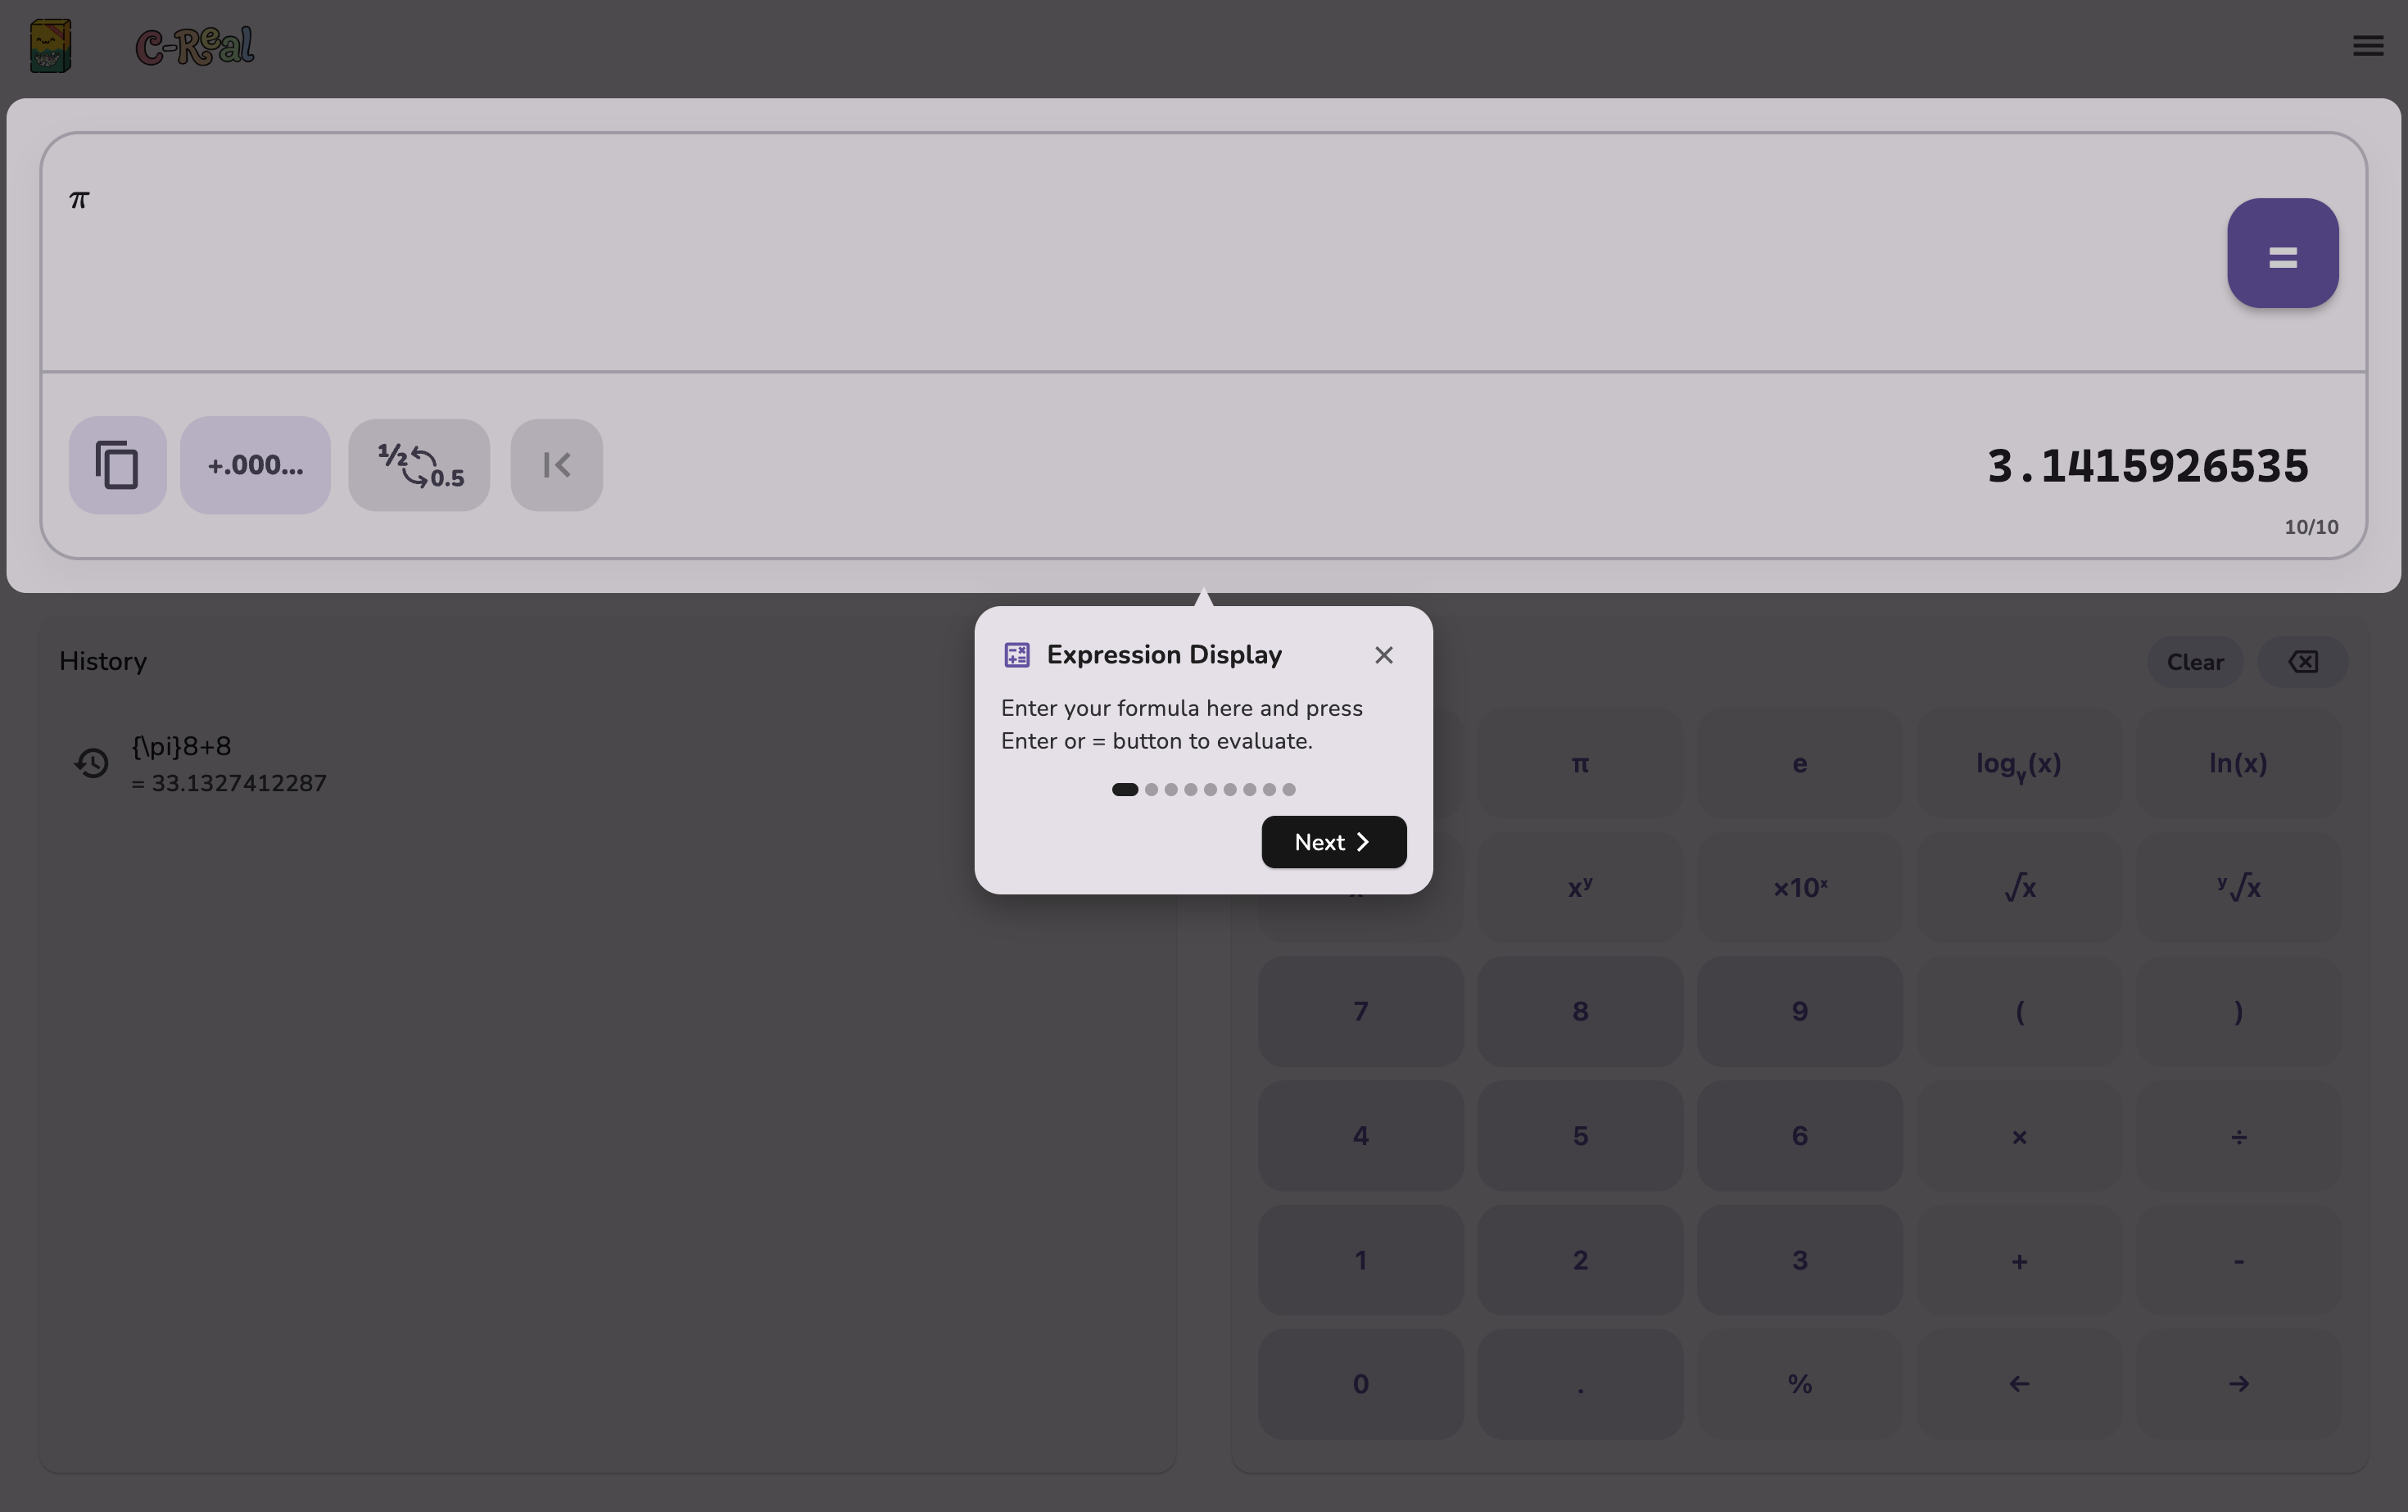
\includegraphics[width=0.6\textwidth]{images/first.png}
    \caption{Vstupní pole}
    \label{fig:expression-display}
\end{figure}

Do vstupního pole uživatel zadává matematický výraz, který chce vypočítat.

Výrazy lze zapisovat pomocí fyzické klávesnice i prostřednictvím tlačítek aplikace. Výpočet se provádí automaticky, stisknutím tlačítka \(=\) se zapíše do historie.

\subsection{Klávesnice}

\begin{figure}[H]
    \centering
    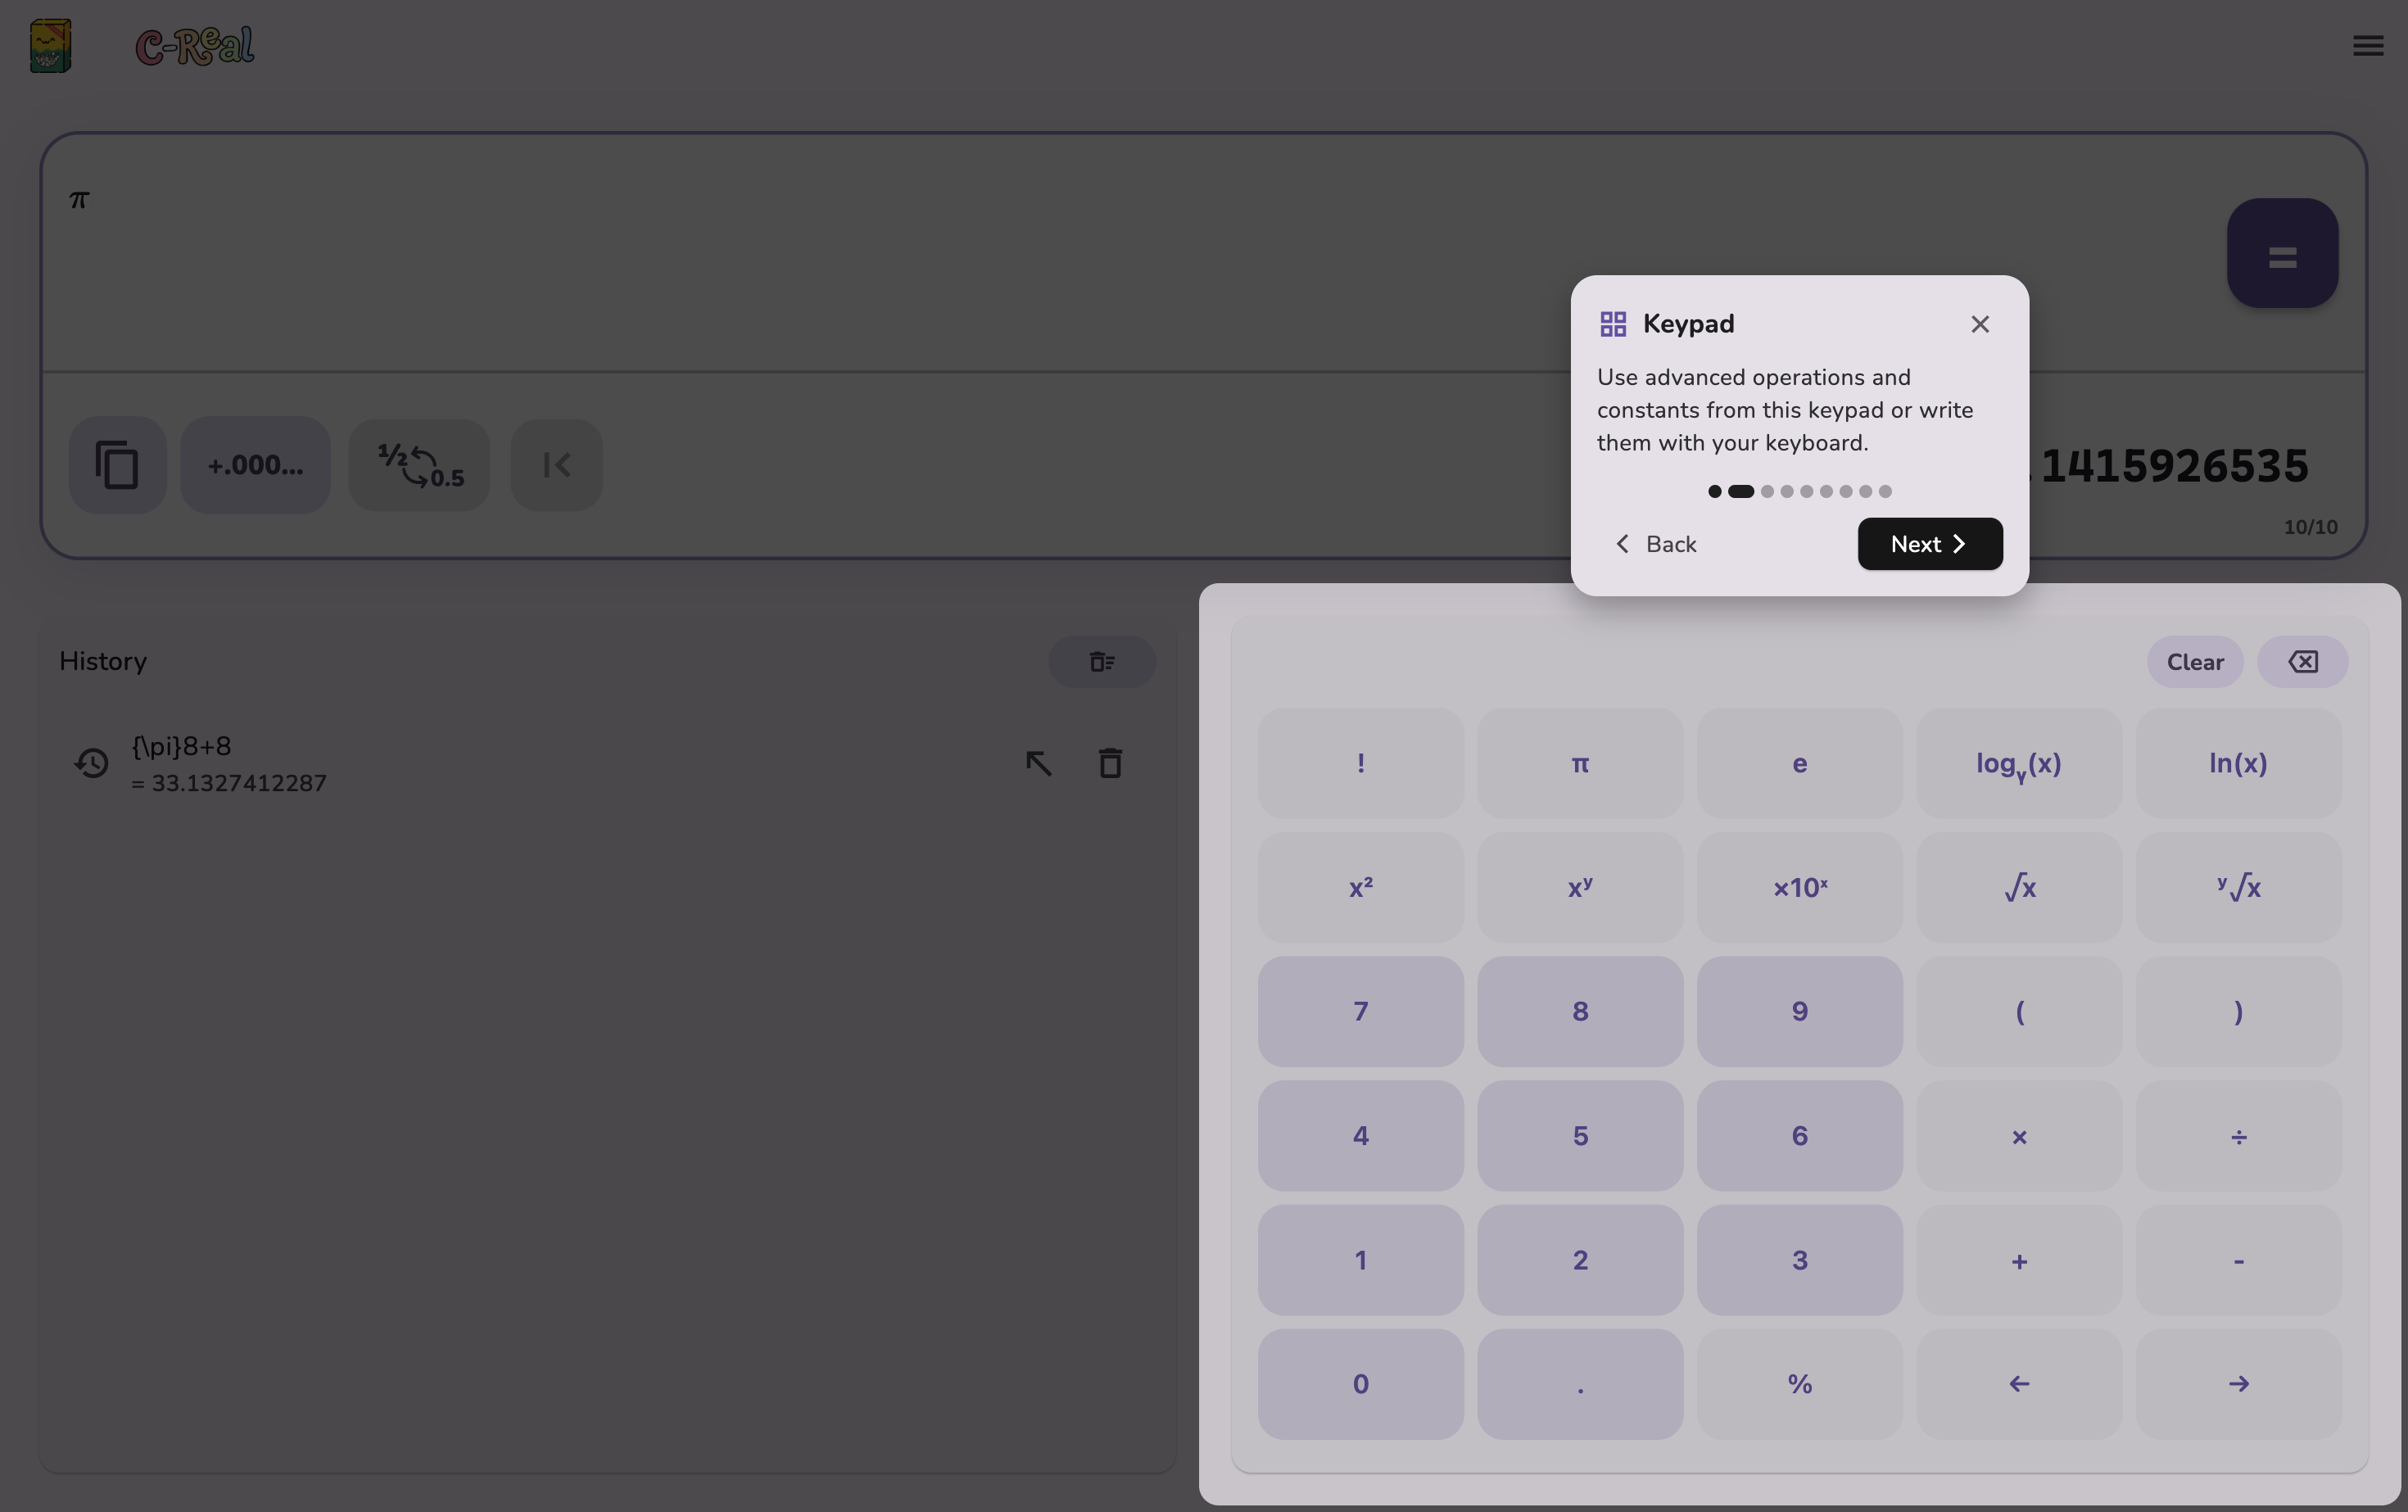
\includegraphics[width=0.6\textwidth]{images/second.png}
    \caption{Klávesnice}
    \label{fig:keypad}
\end{figure}

Klávesnice aplikace umožňuje rychlé vkládání matematických operací, funkcí a konstant bez nutnosti jejich ručního vypisování. Uživatel tak může jednoduše zadávat i složitější výrazy.

\subsection{Kopírování výsledku}

\begin{figure}[H]
    \centering
    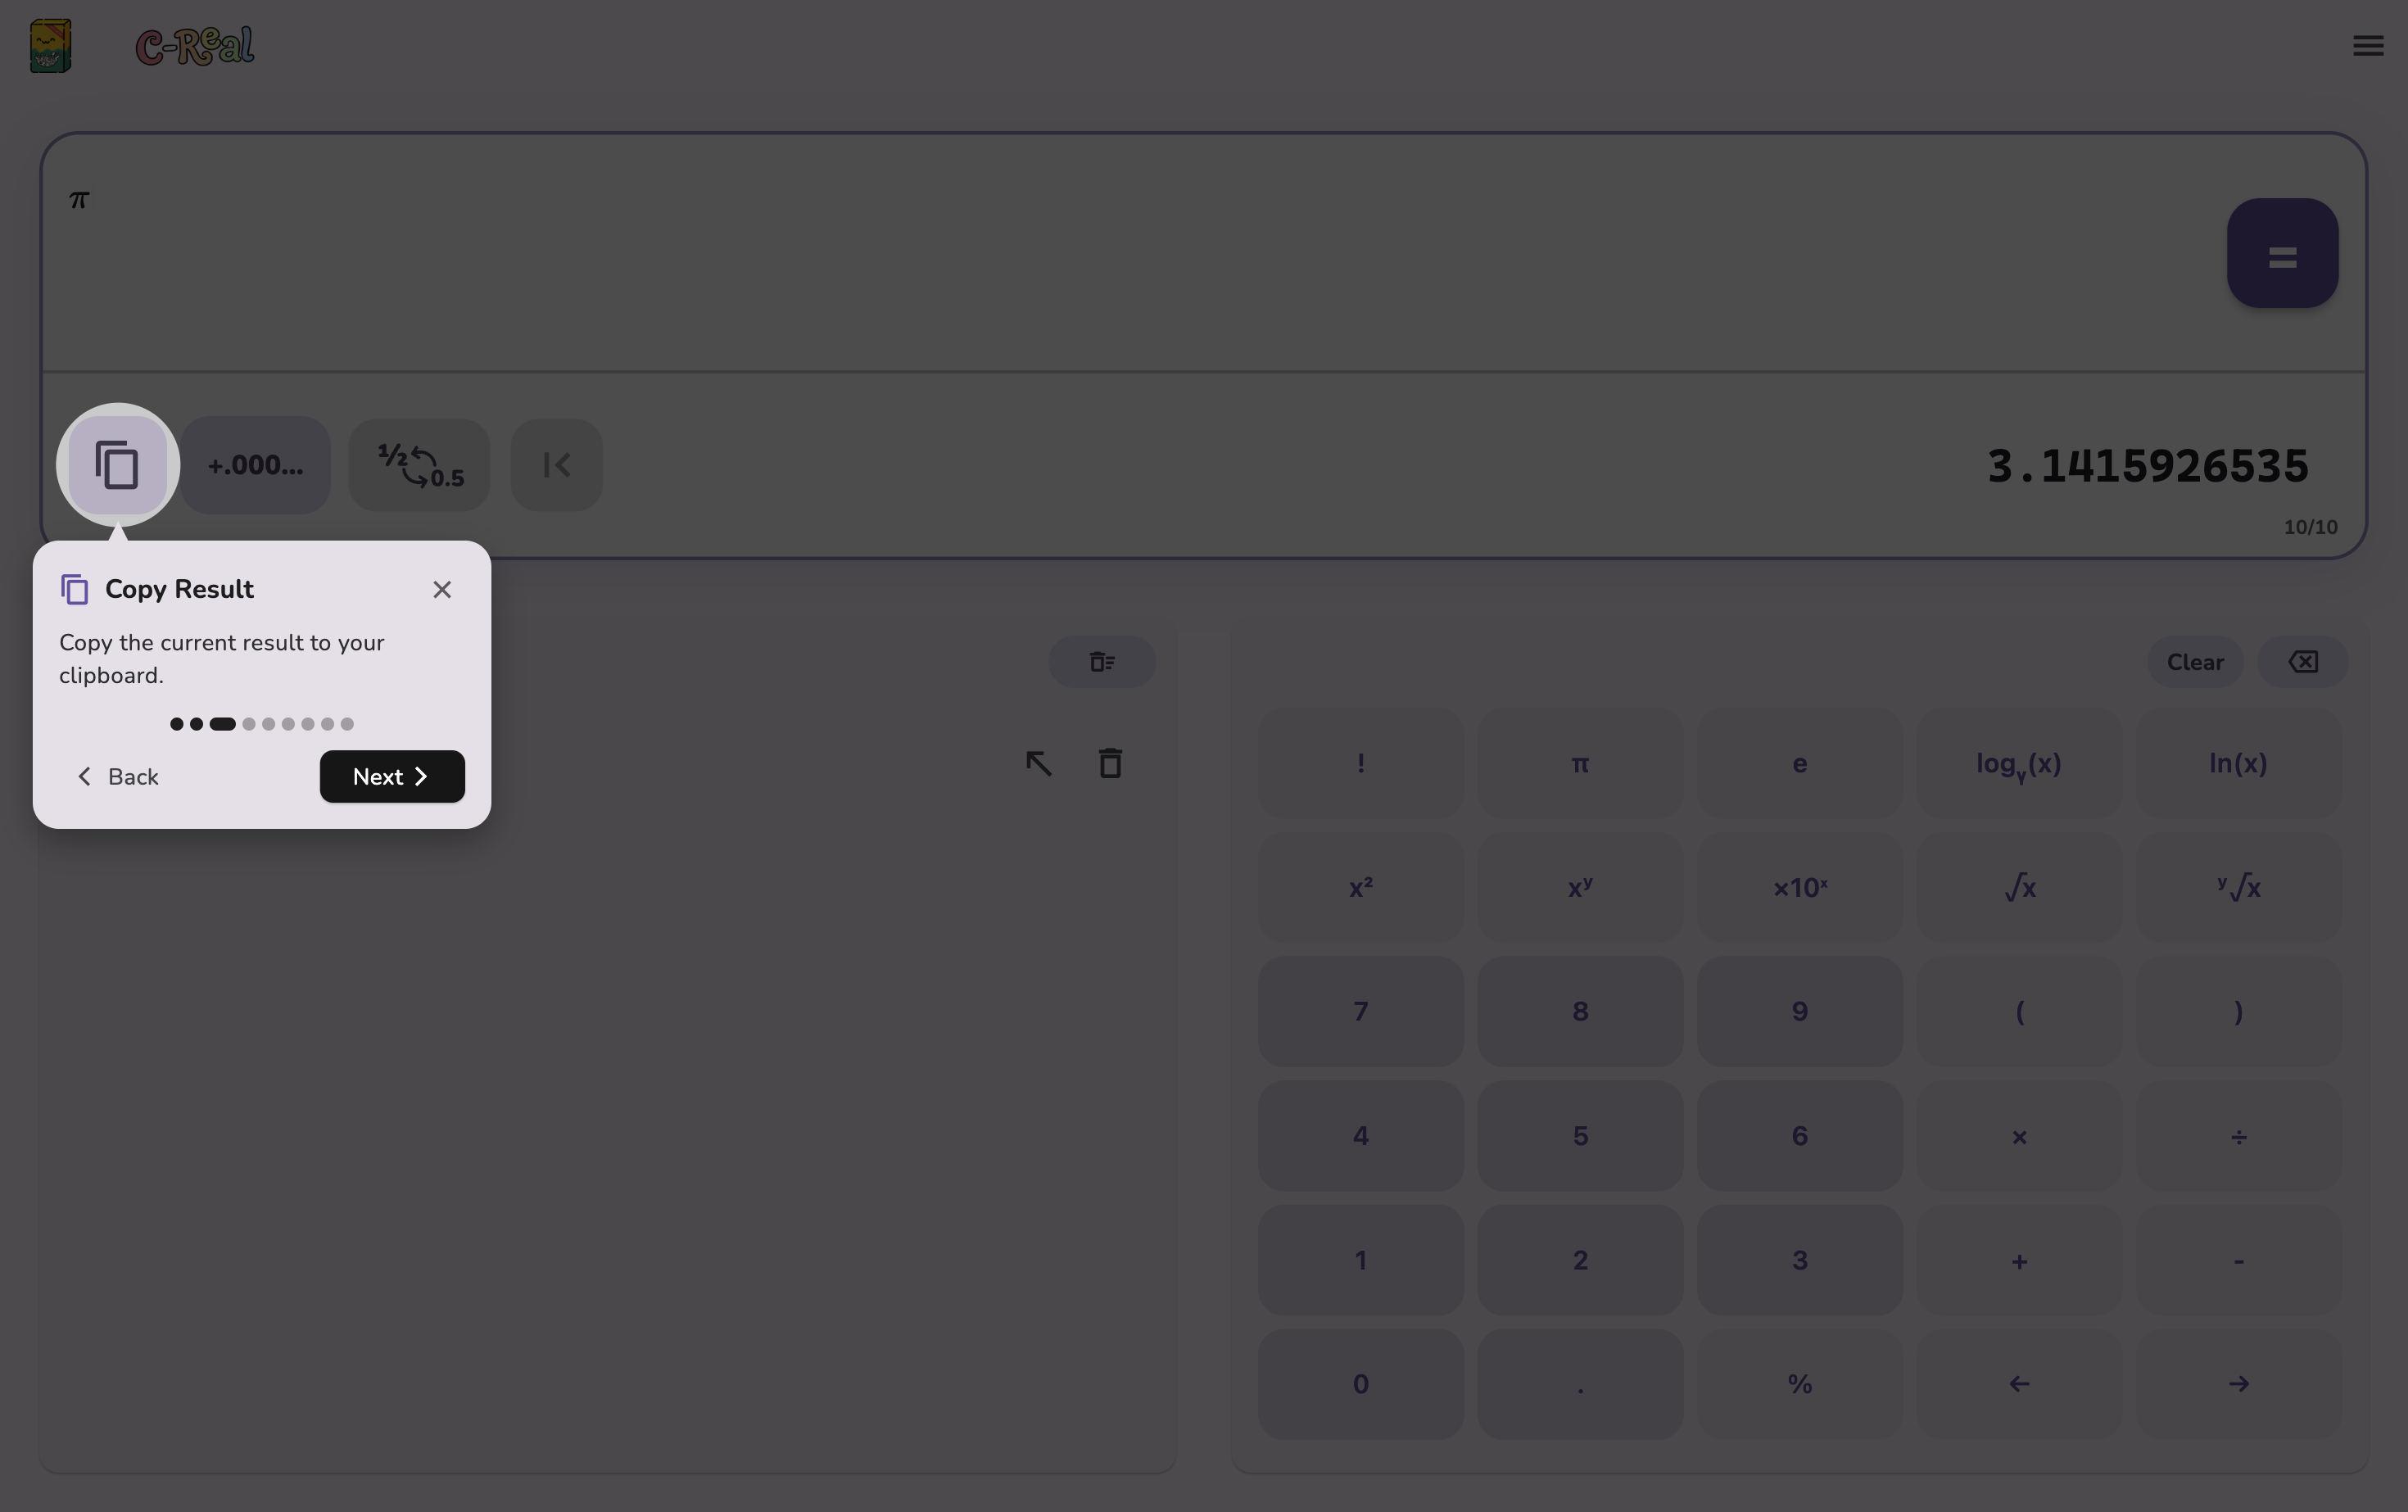
\includegraphics[width=0.6\textwidth]{images/third.png}
    \caption{Tlačitko pro kopírování výsledku}
    \label{fig:copy-result}
\end{figure}

Toto tlačítko slouží ke zkopírování aktuálně zobrazeného výsledku do schránky. Uživatel může následně výsledek vložit do jiné aplikace nebo dokumentu.

\subsection{Zvýšení přesnosti výsledku}

\begin{figure}[H]
    \centering
    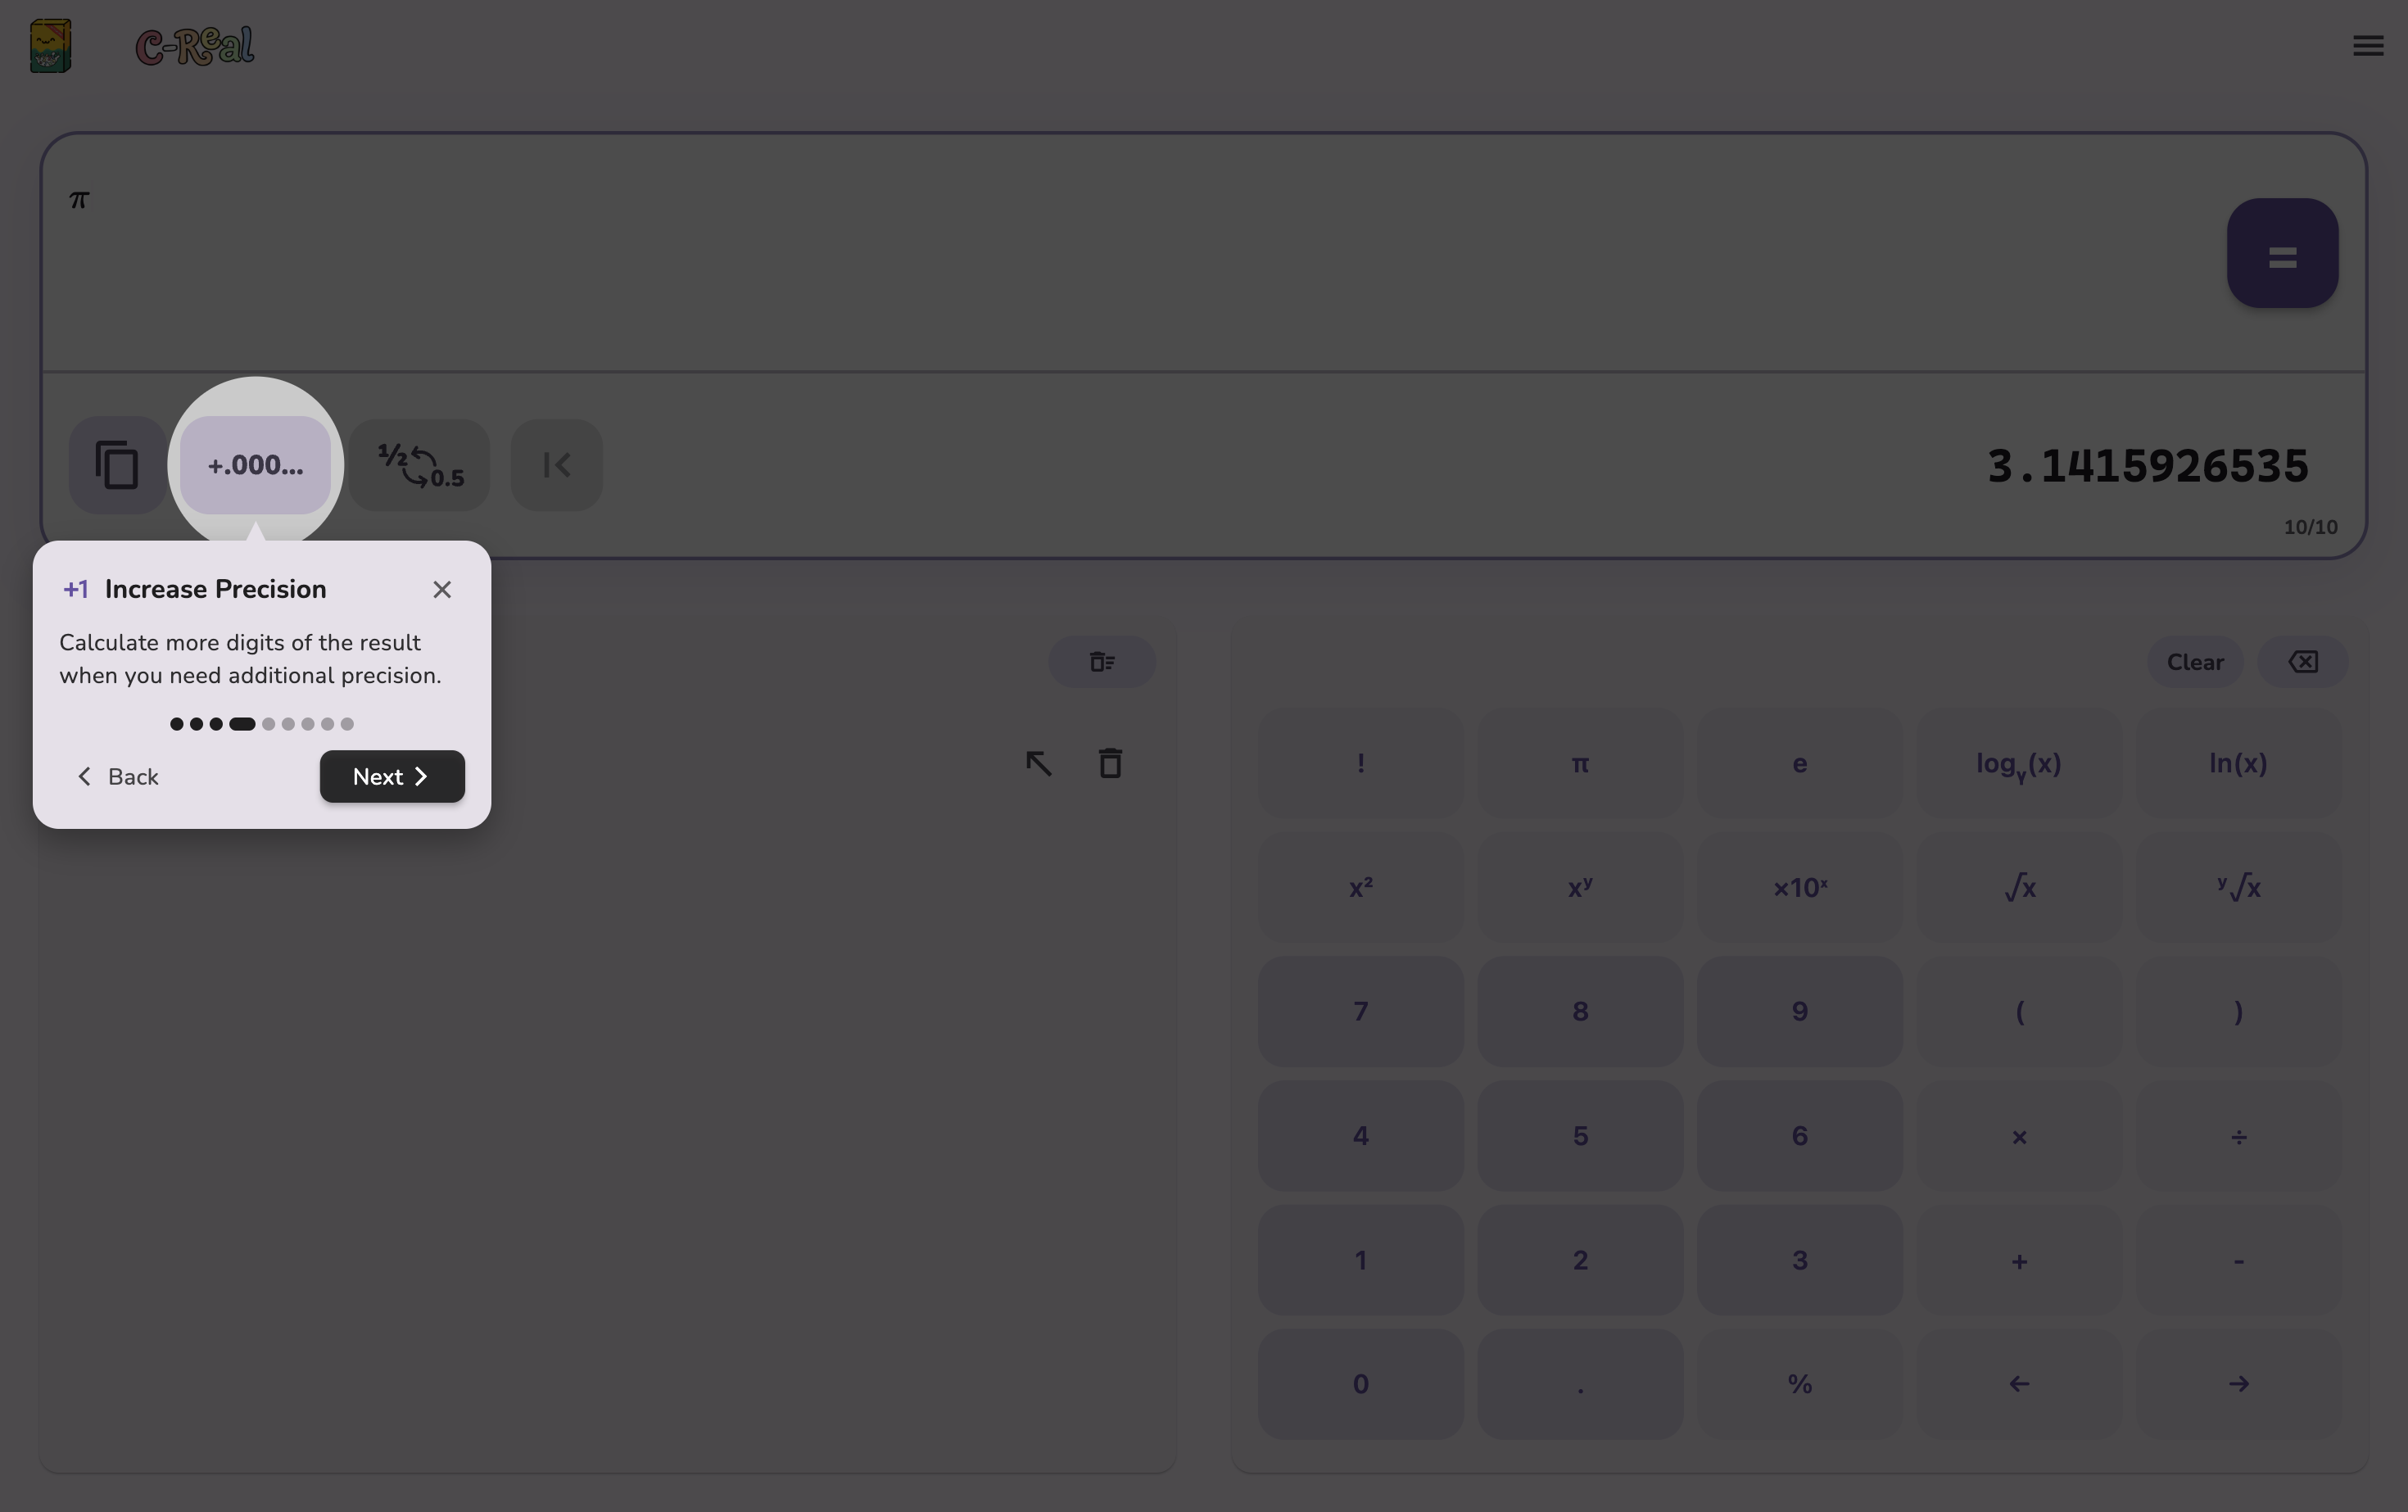
\includegraphics[width=0.6\textwidth]{images/fourth.png}
    \caption{Tlačitko pro zvýšení přesnosti výsledku}
    \label{fig:increase-precision}
\end{figure}

Funkce zvýšení přesnosti umožňuje vypočítat a zobrazit větší počet číslic výsledku. Je užitečná zejména v případech, kdy je vyžadována vyšší numerická přesnost.

\subsection{Zlomek / Desatinné}

\begin{figure}[H]
    \centering
    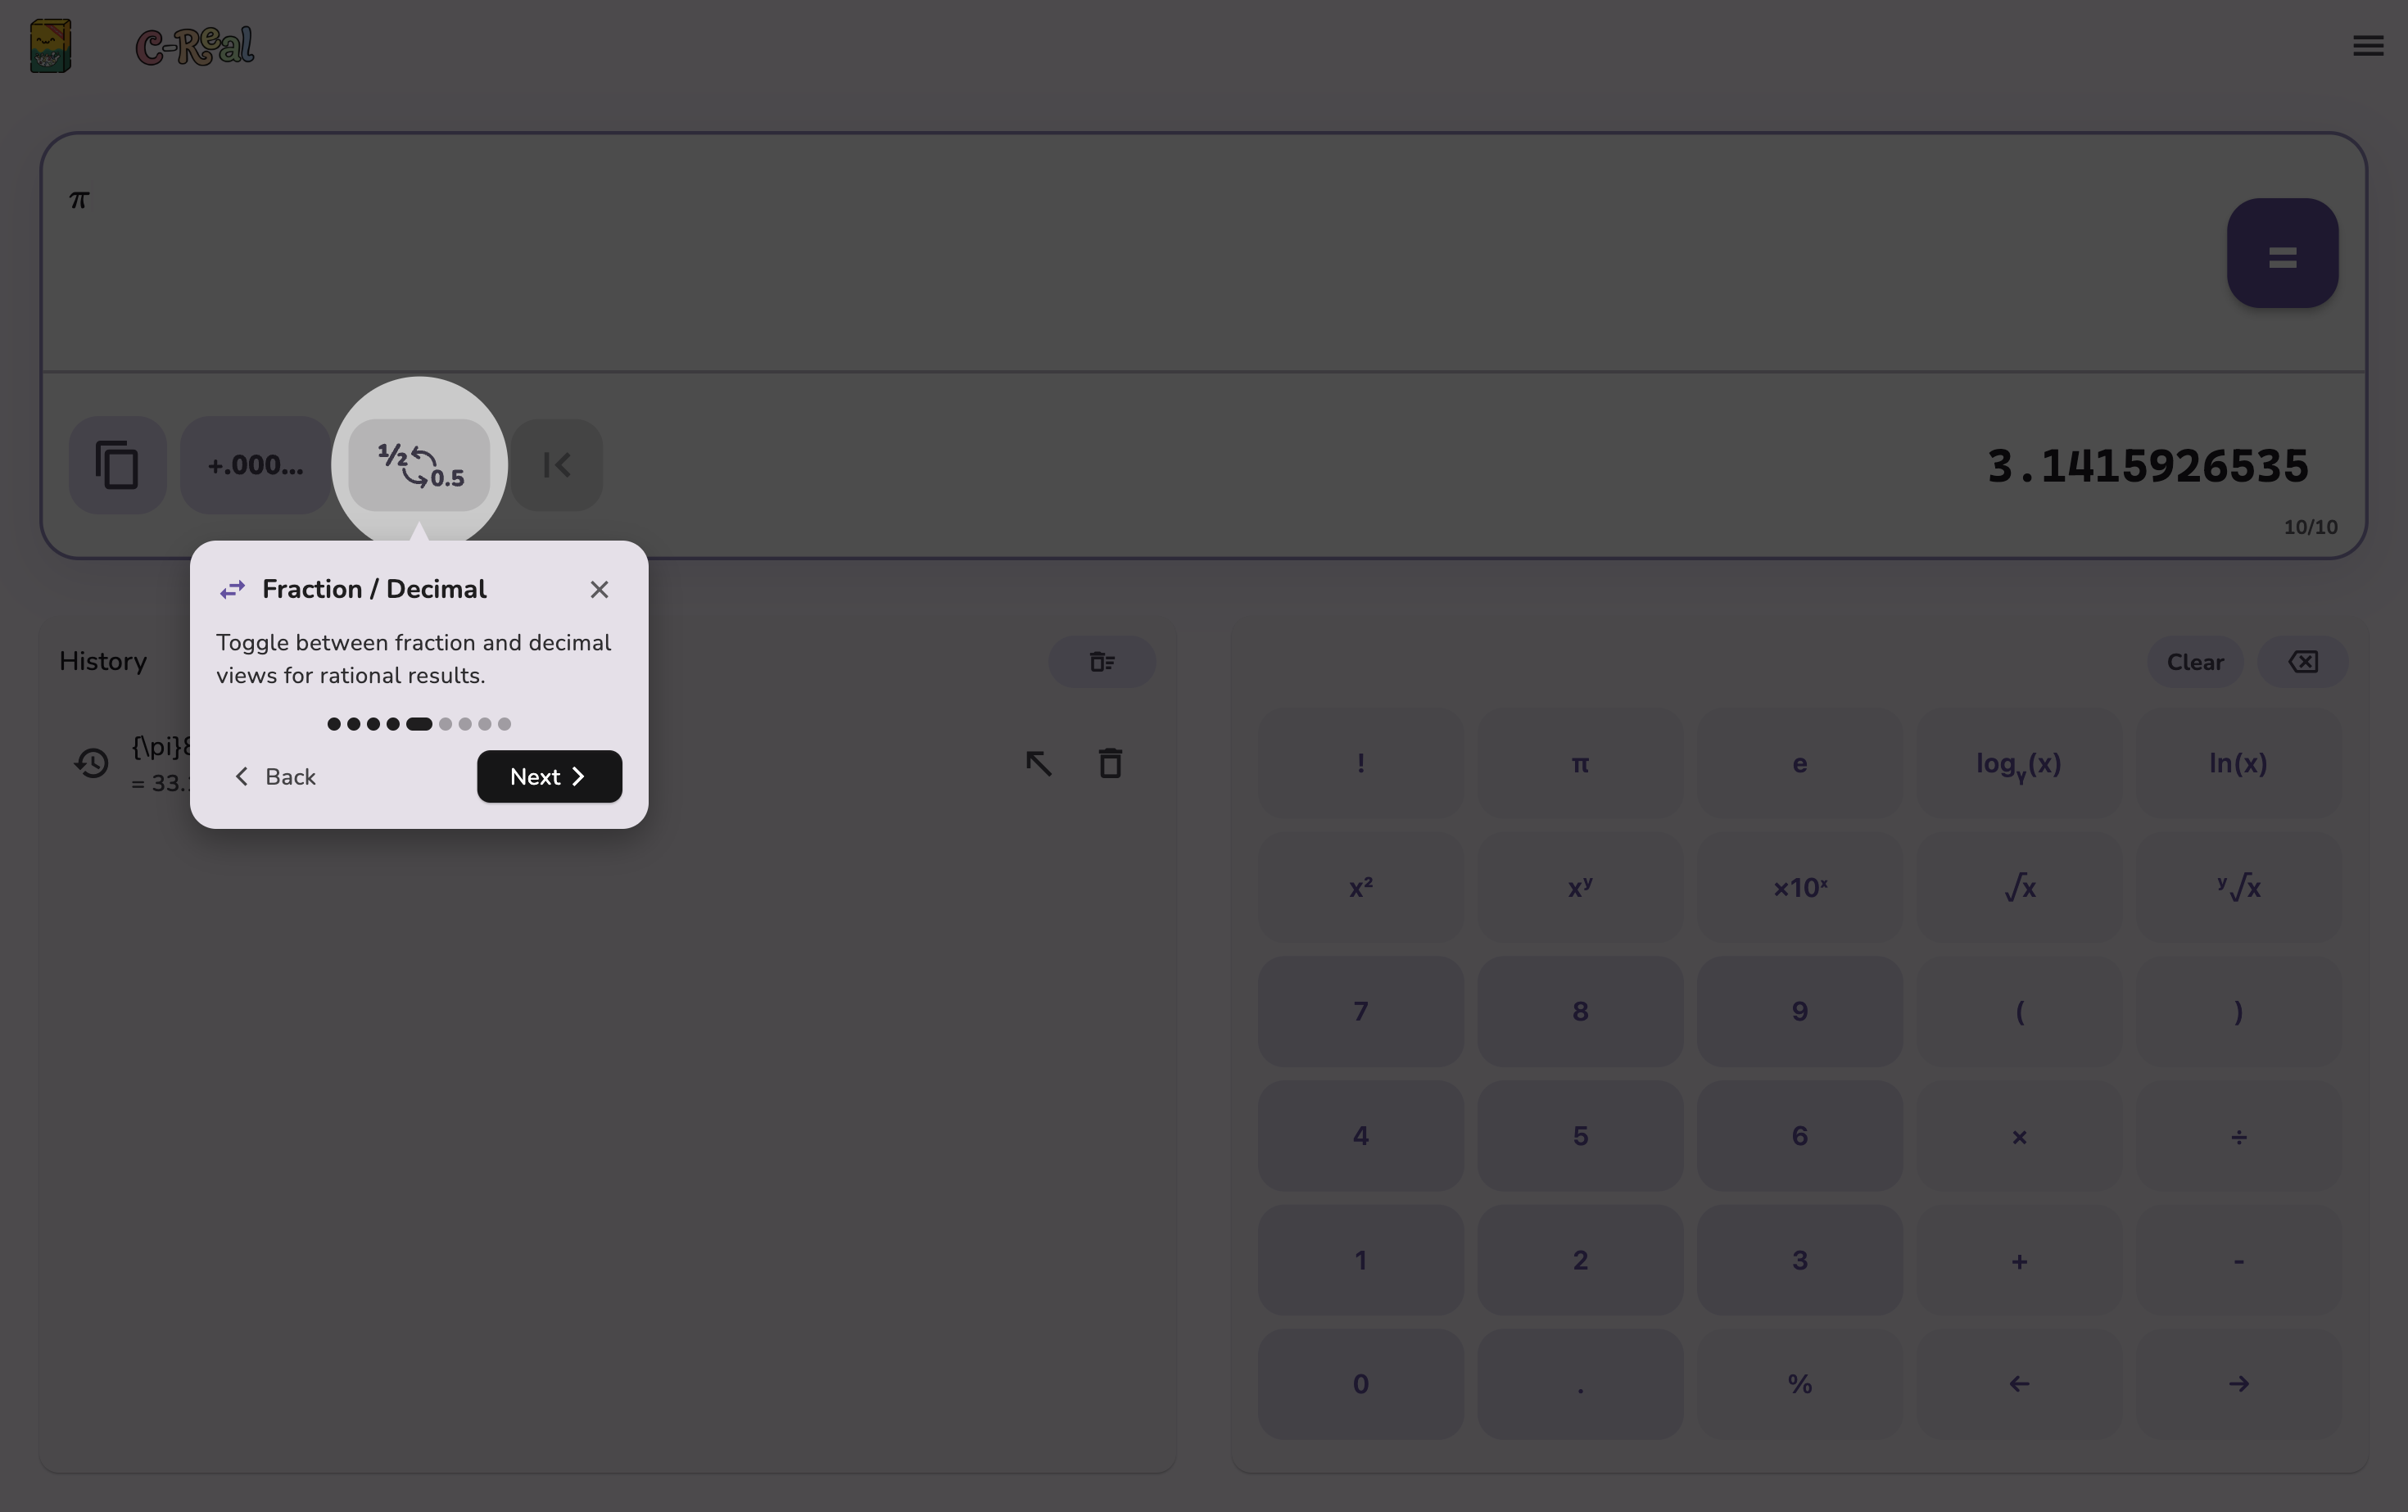
\includegraphics[width=0.6\textwidth]{images/fifth.png}
    \caption{Tlačitko pro převod formátu výsledku}
    \label{fig:fraction-decimal}
\end{figure}

U racionálních výsledků je možné přepínat mezi zlomkovým tvarem a desetinným vyjádřením. Tato funkcionalita poskytuje uživateli větší flexibilitu při interpretaci výsledku.

\subsection{Posun na začátek výsledku}

\begin{figure}[H]
    \centering
    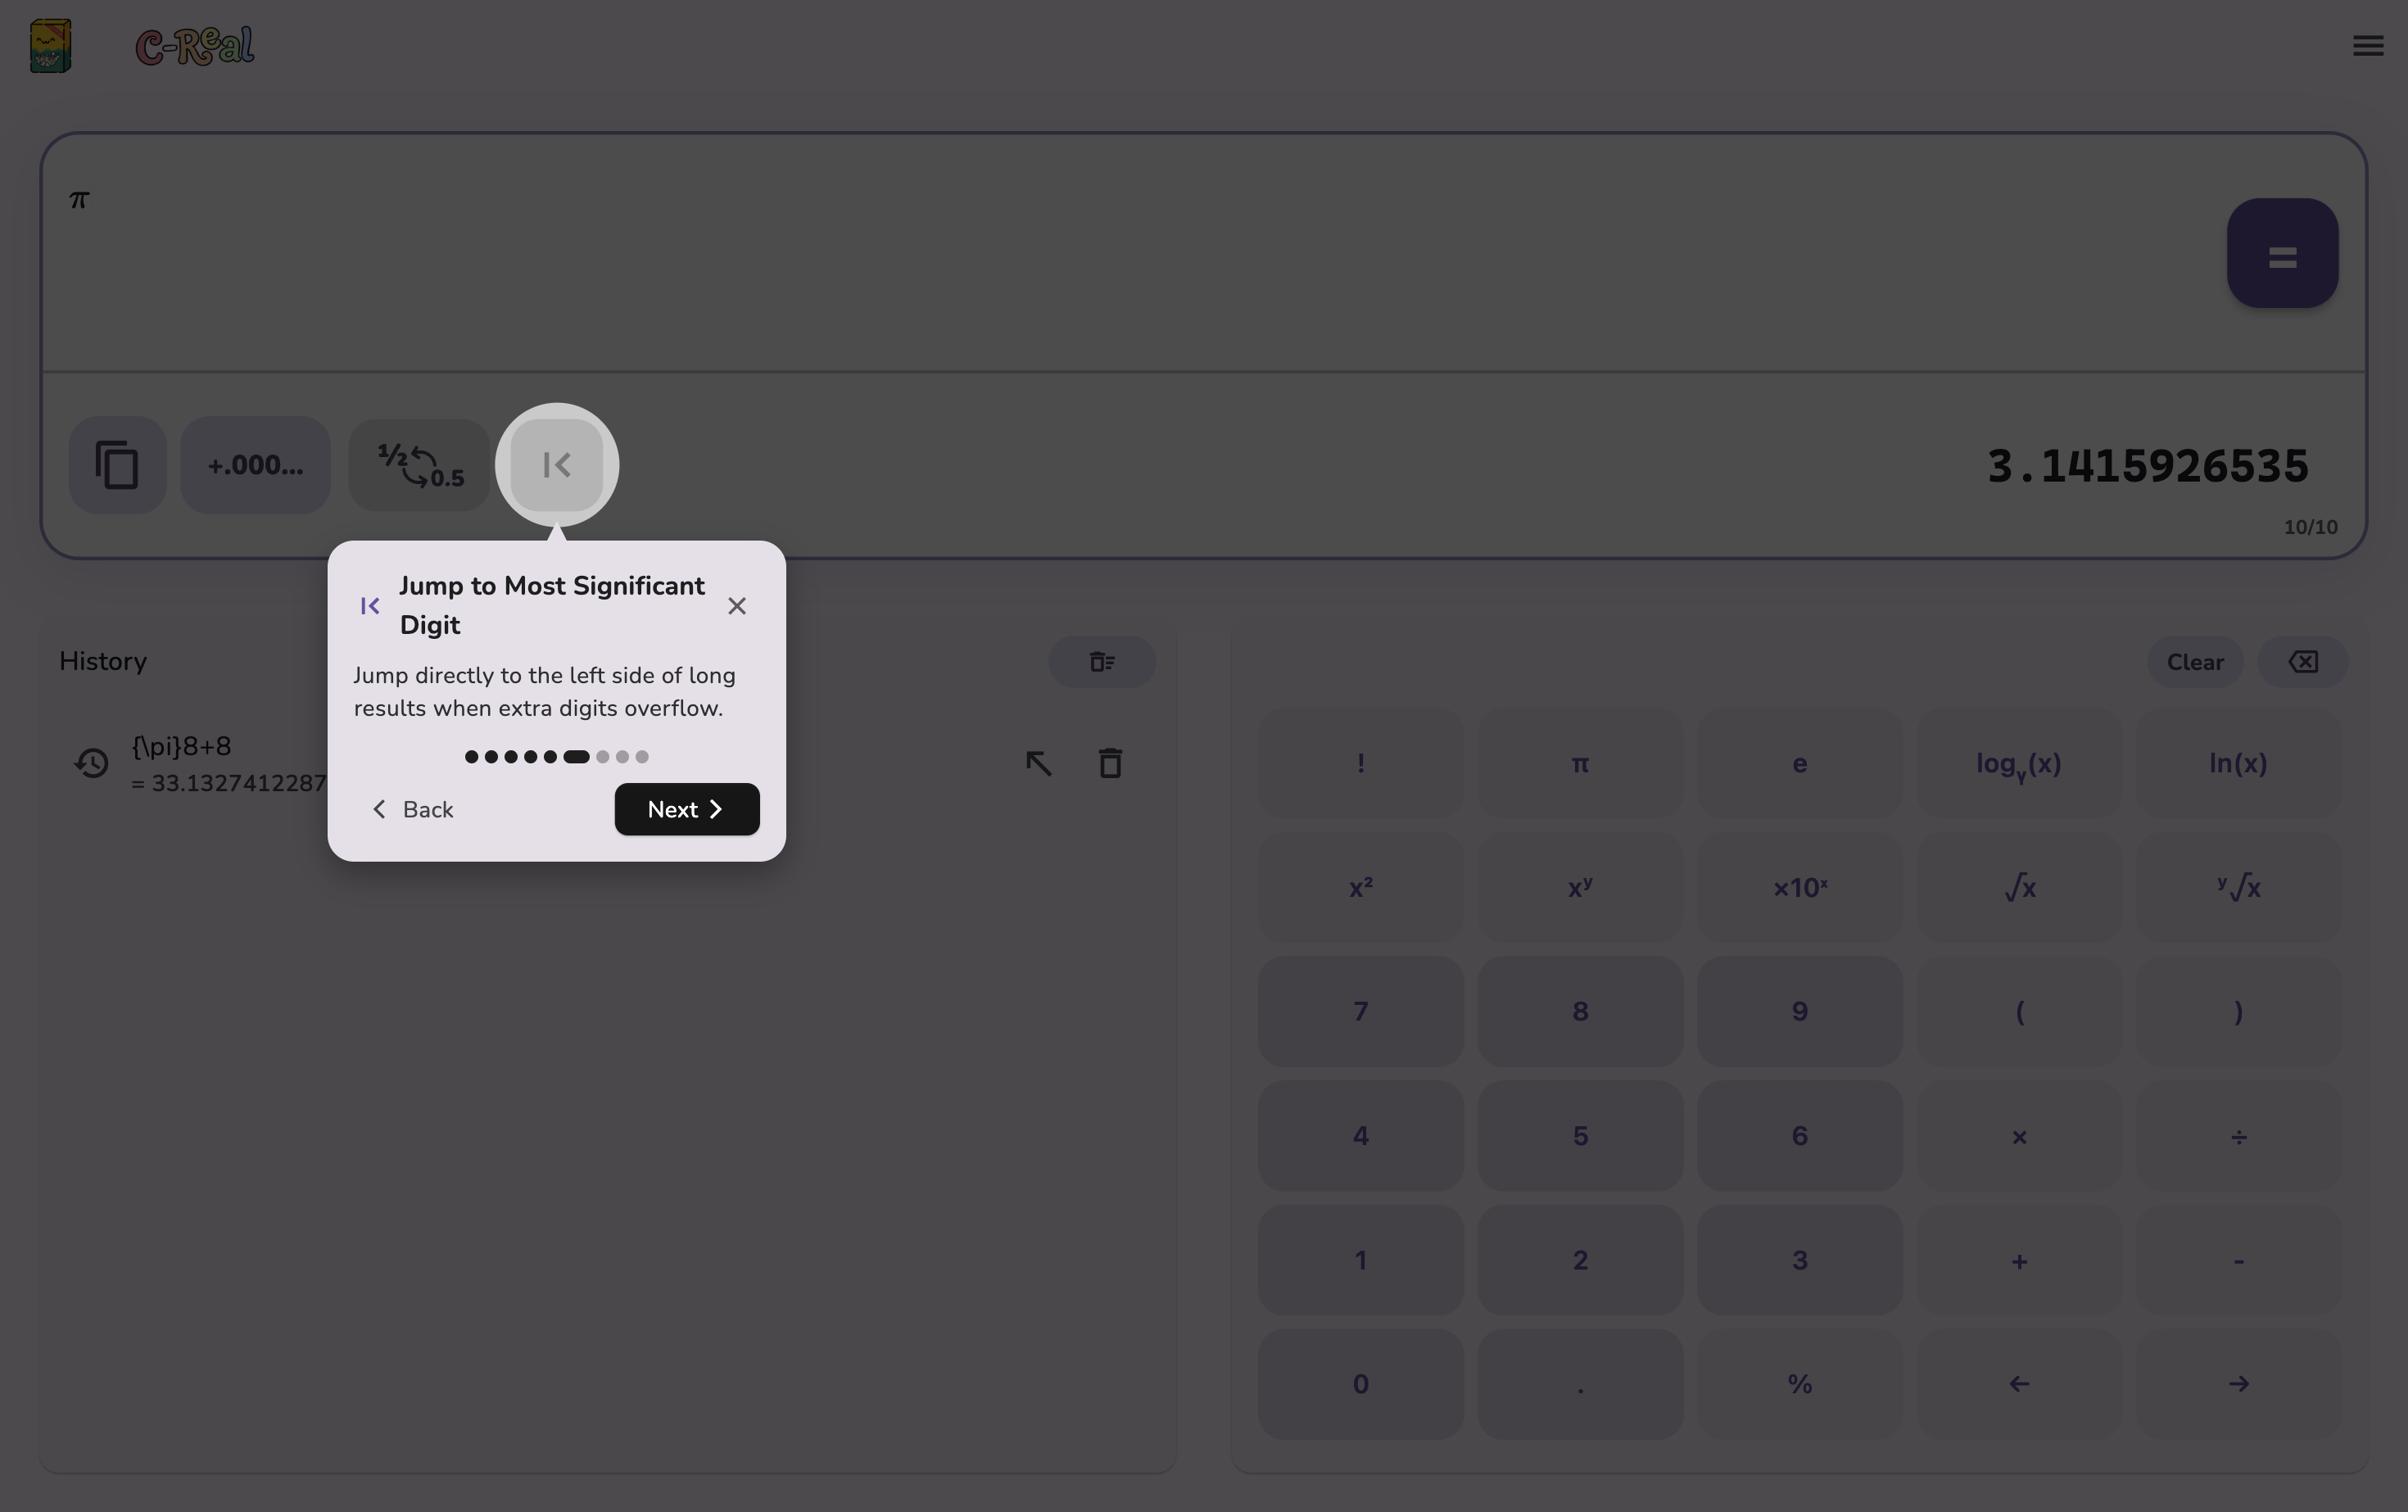
\includegraphics[width=0.6\textwidth]{images/sixth.png}
    \caption{Tlačitko pro skok na první číslici výsledku}
    \label{fig:jump-most-significant-digit}
\end{figure}

U dlouhých výsledků umožňuje tato funkce okamžitý přesun na začátek čísla, tedy k jeho nejvýznamnější číslici. Uživatel tak nemusí výsledek ručně posouvat zpět na jeho začátek.

\subsection{Pole výsledku}

\begin{figure}[H]
    \centering
    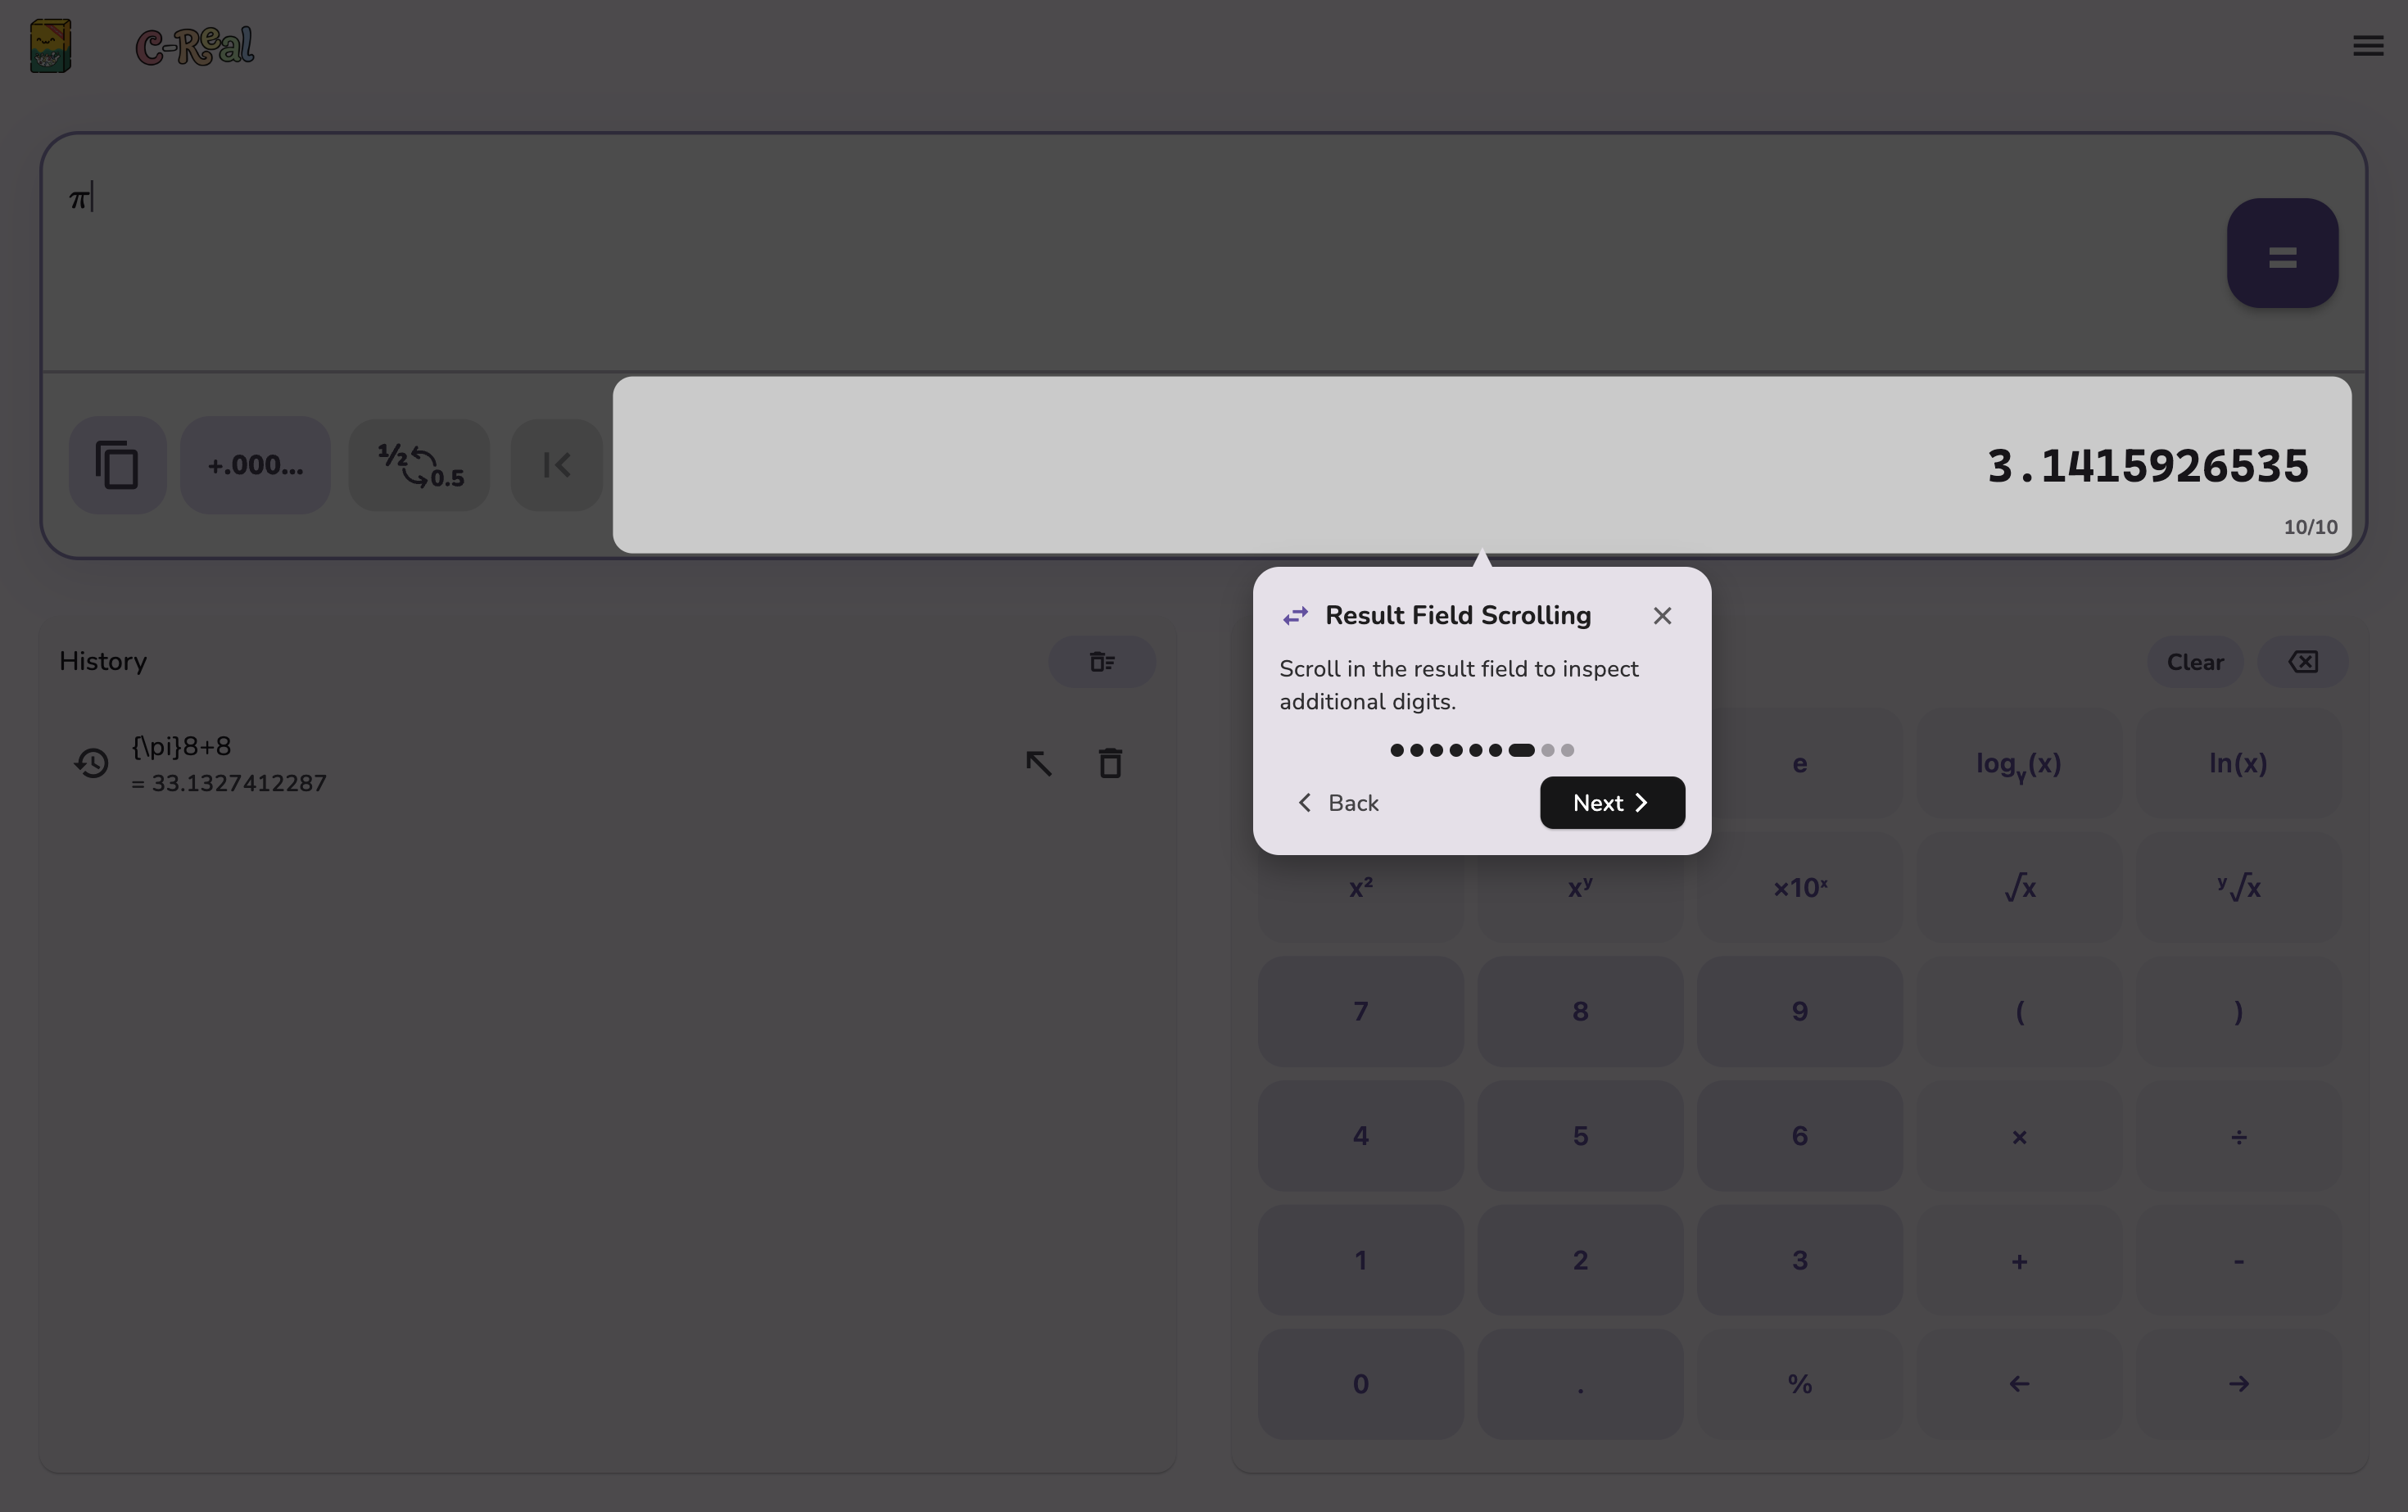
\includegraphics[width=0.6\textwidth]{images/seventh.png}
    \caption{Pole výsledku}
    \label{fig:result-field-scrolling}
\end{figure}

Pokud je výsledek příliš dlouhý na zobrazení v celém rozsahu, může se uživatel ve výsledkovém poli posouvat kolečkem myši a prohlížet si další číslice. Tato funkce je užitečná zejména při práci s dlouhými desetinnými čísly.

\subsection{Historie}

\begin{figure}[H]
    \centering
    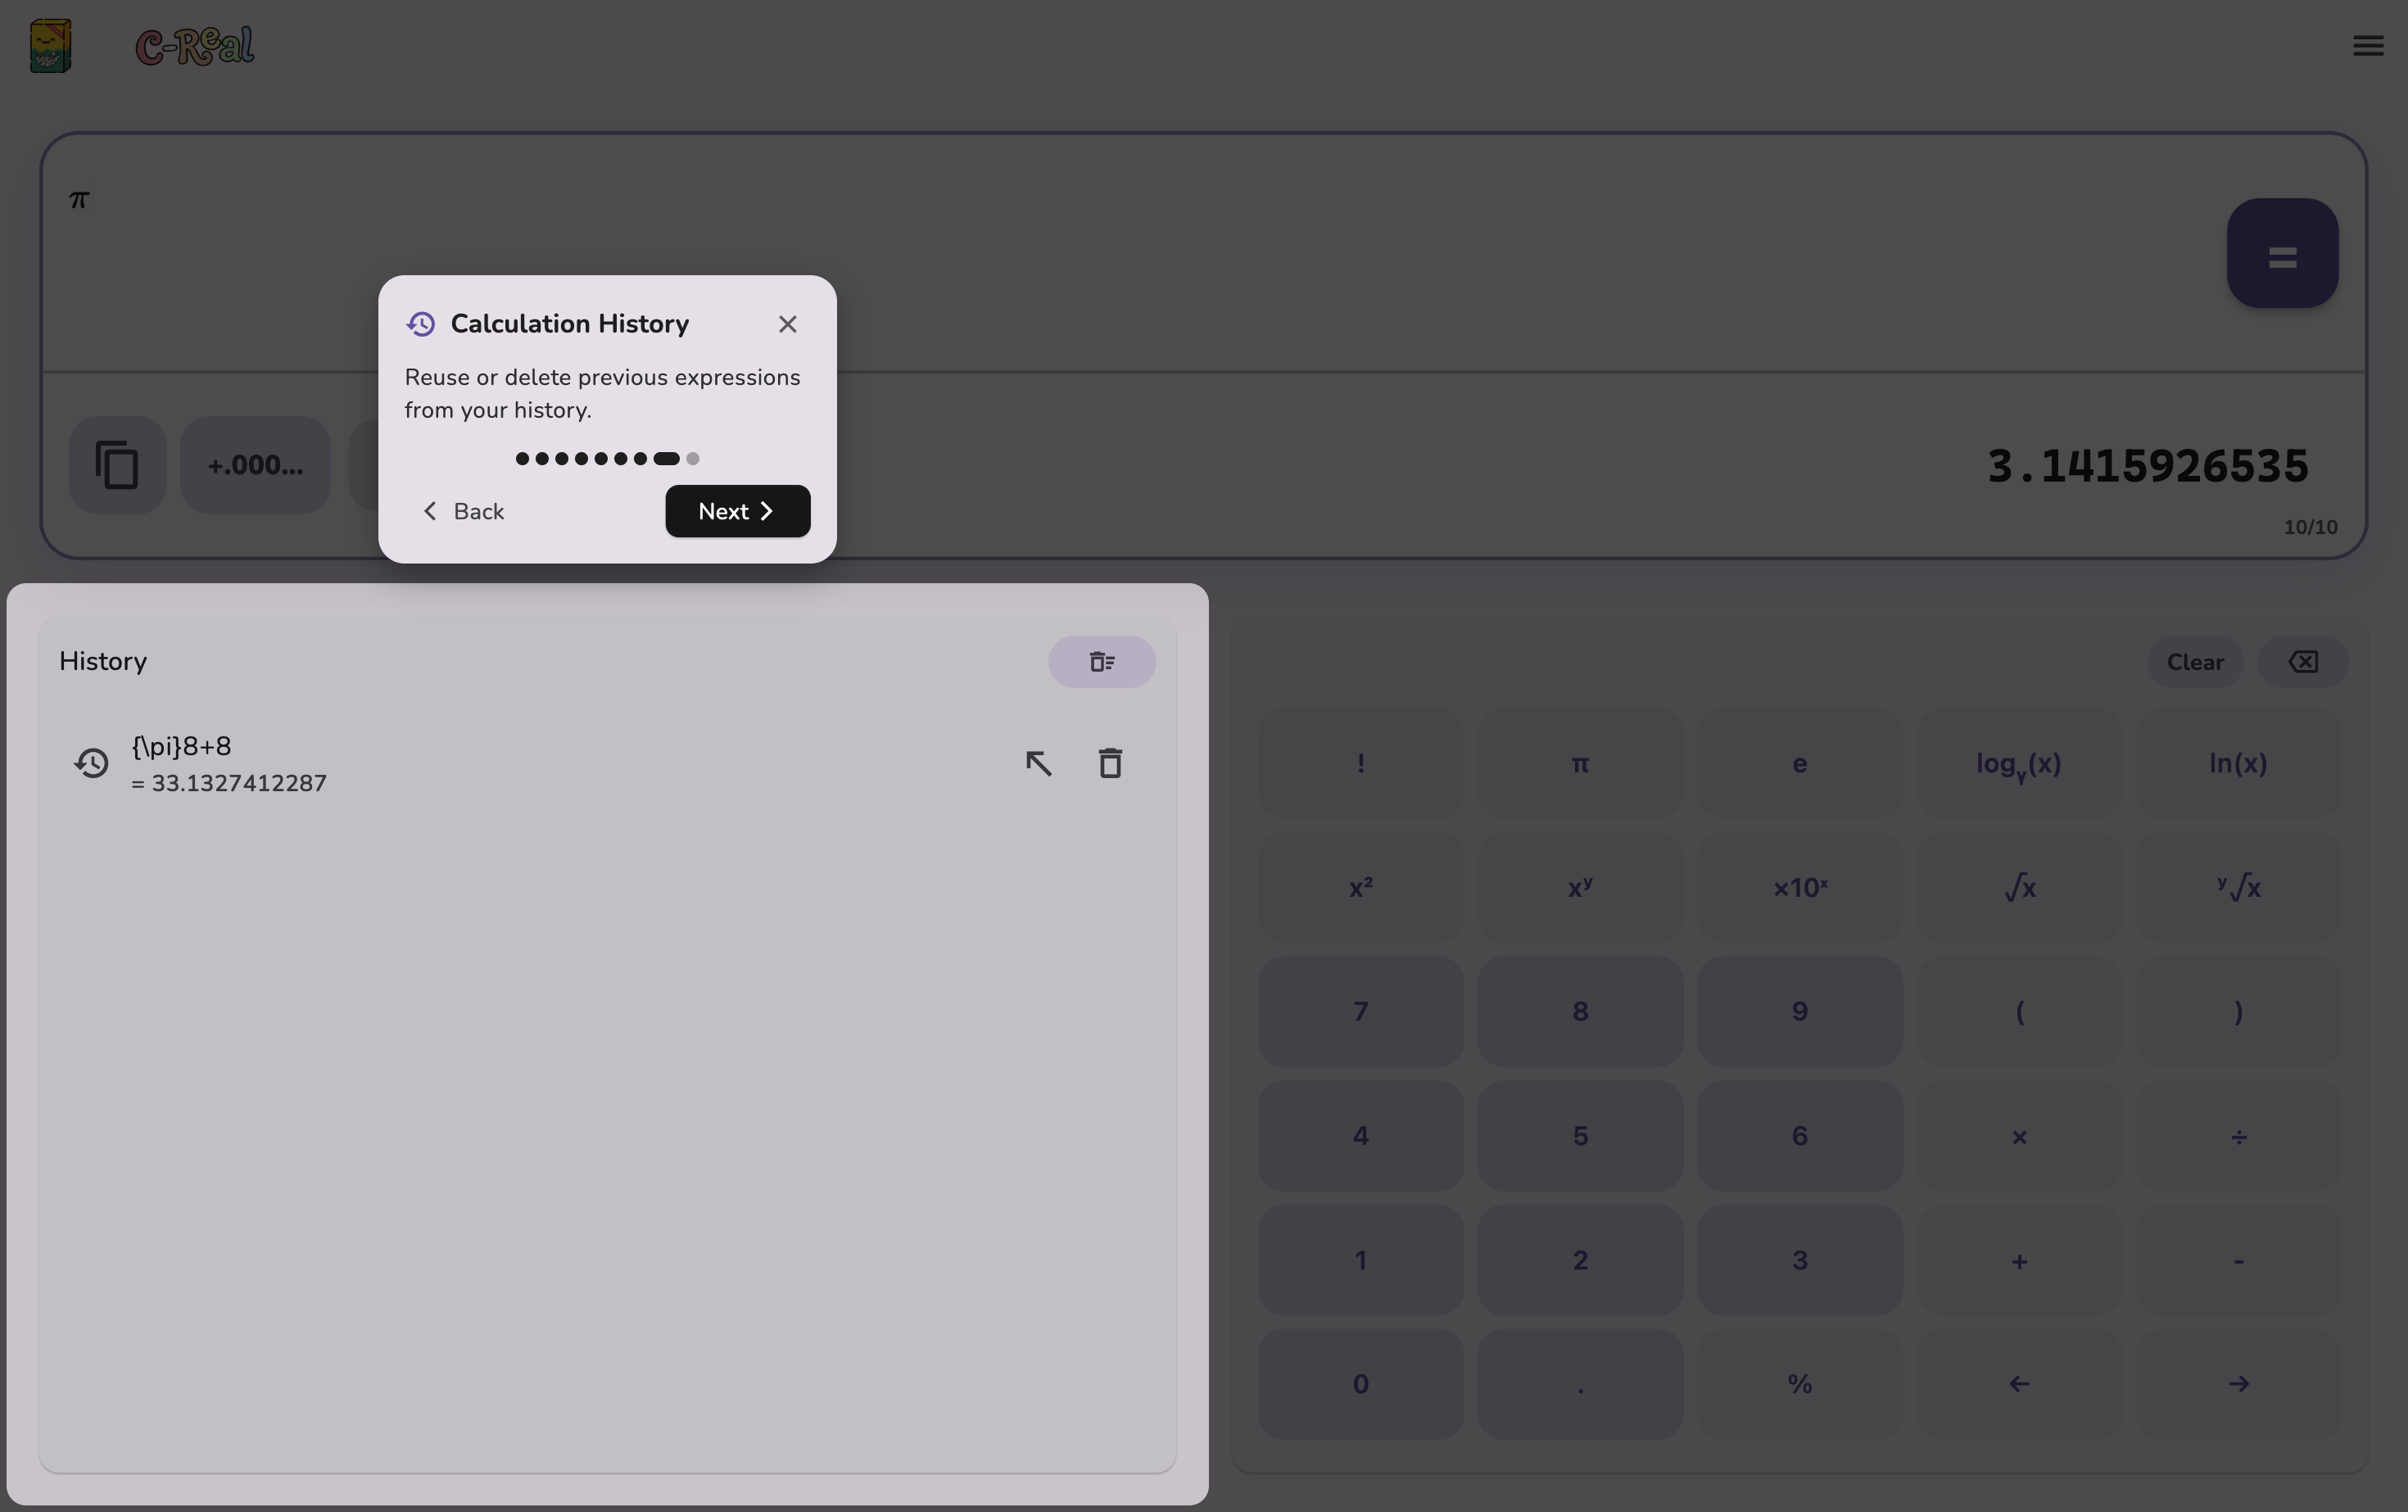
\includegraphics[width=0.6\textwidth]{images/eighth.png}
    \caption{Historie}
    \label{fig:calculation-history}
\end{figure}

Historie výpočtů uchovává dříve zadané výrazy a jejich výsledky. Uživatel je může kliknutím znovu použít nebo je odstranit, pokud již nejsou potřeba.

\subsection{Informace}

\begin{figure}[H]
    \centering
    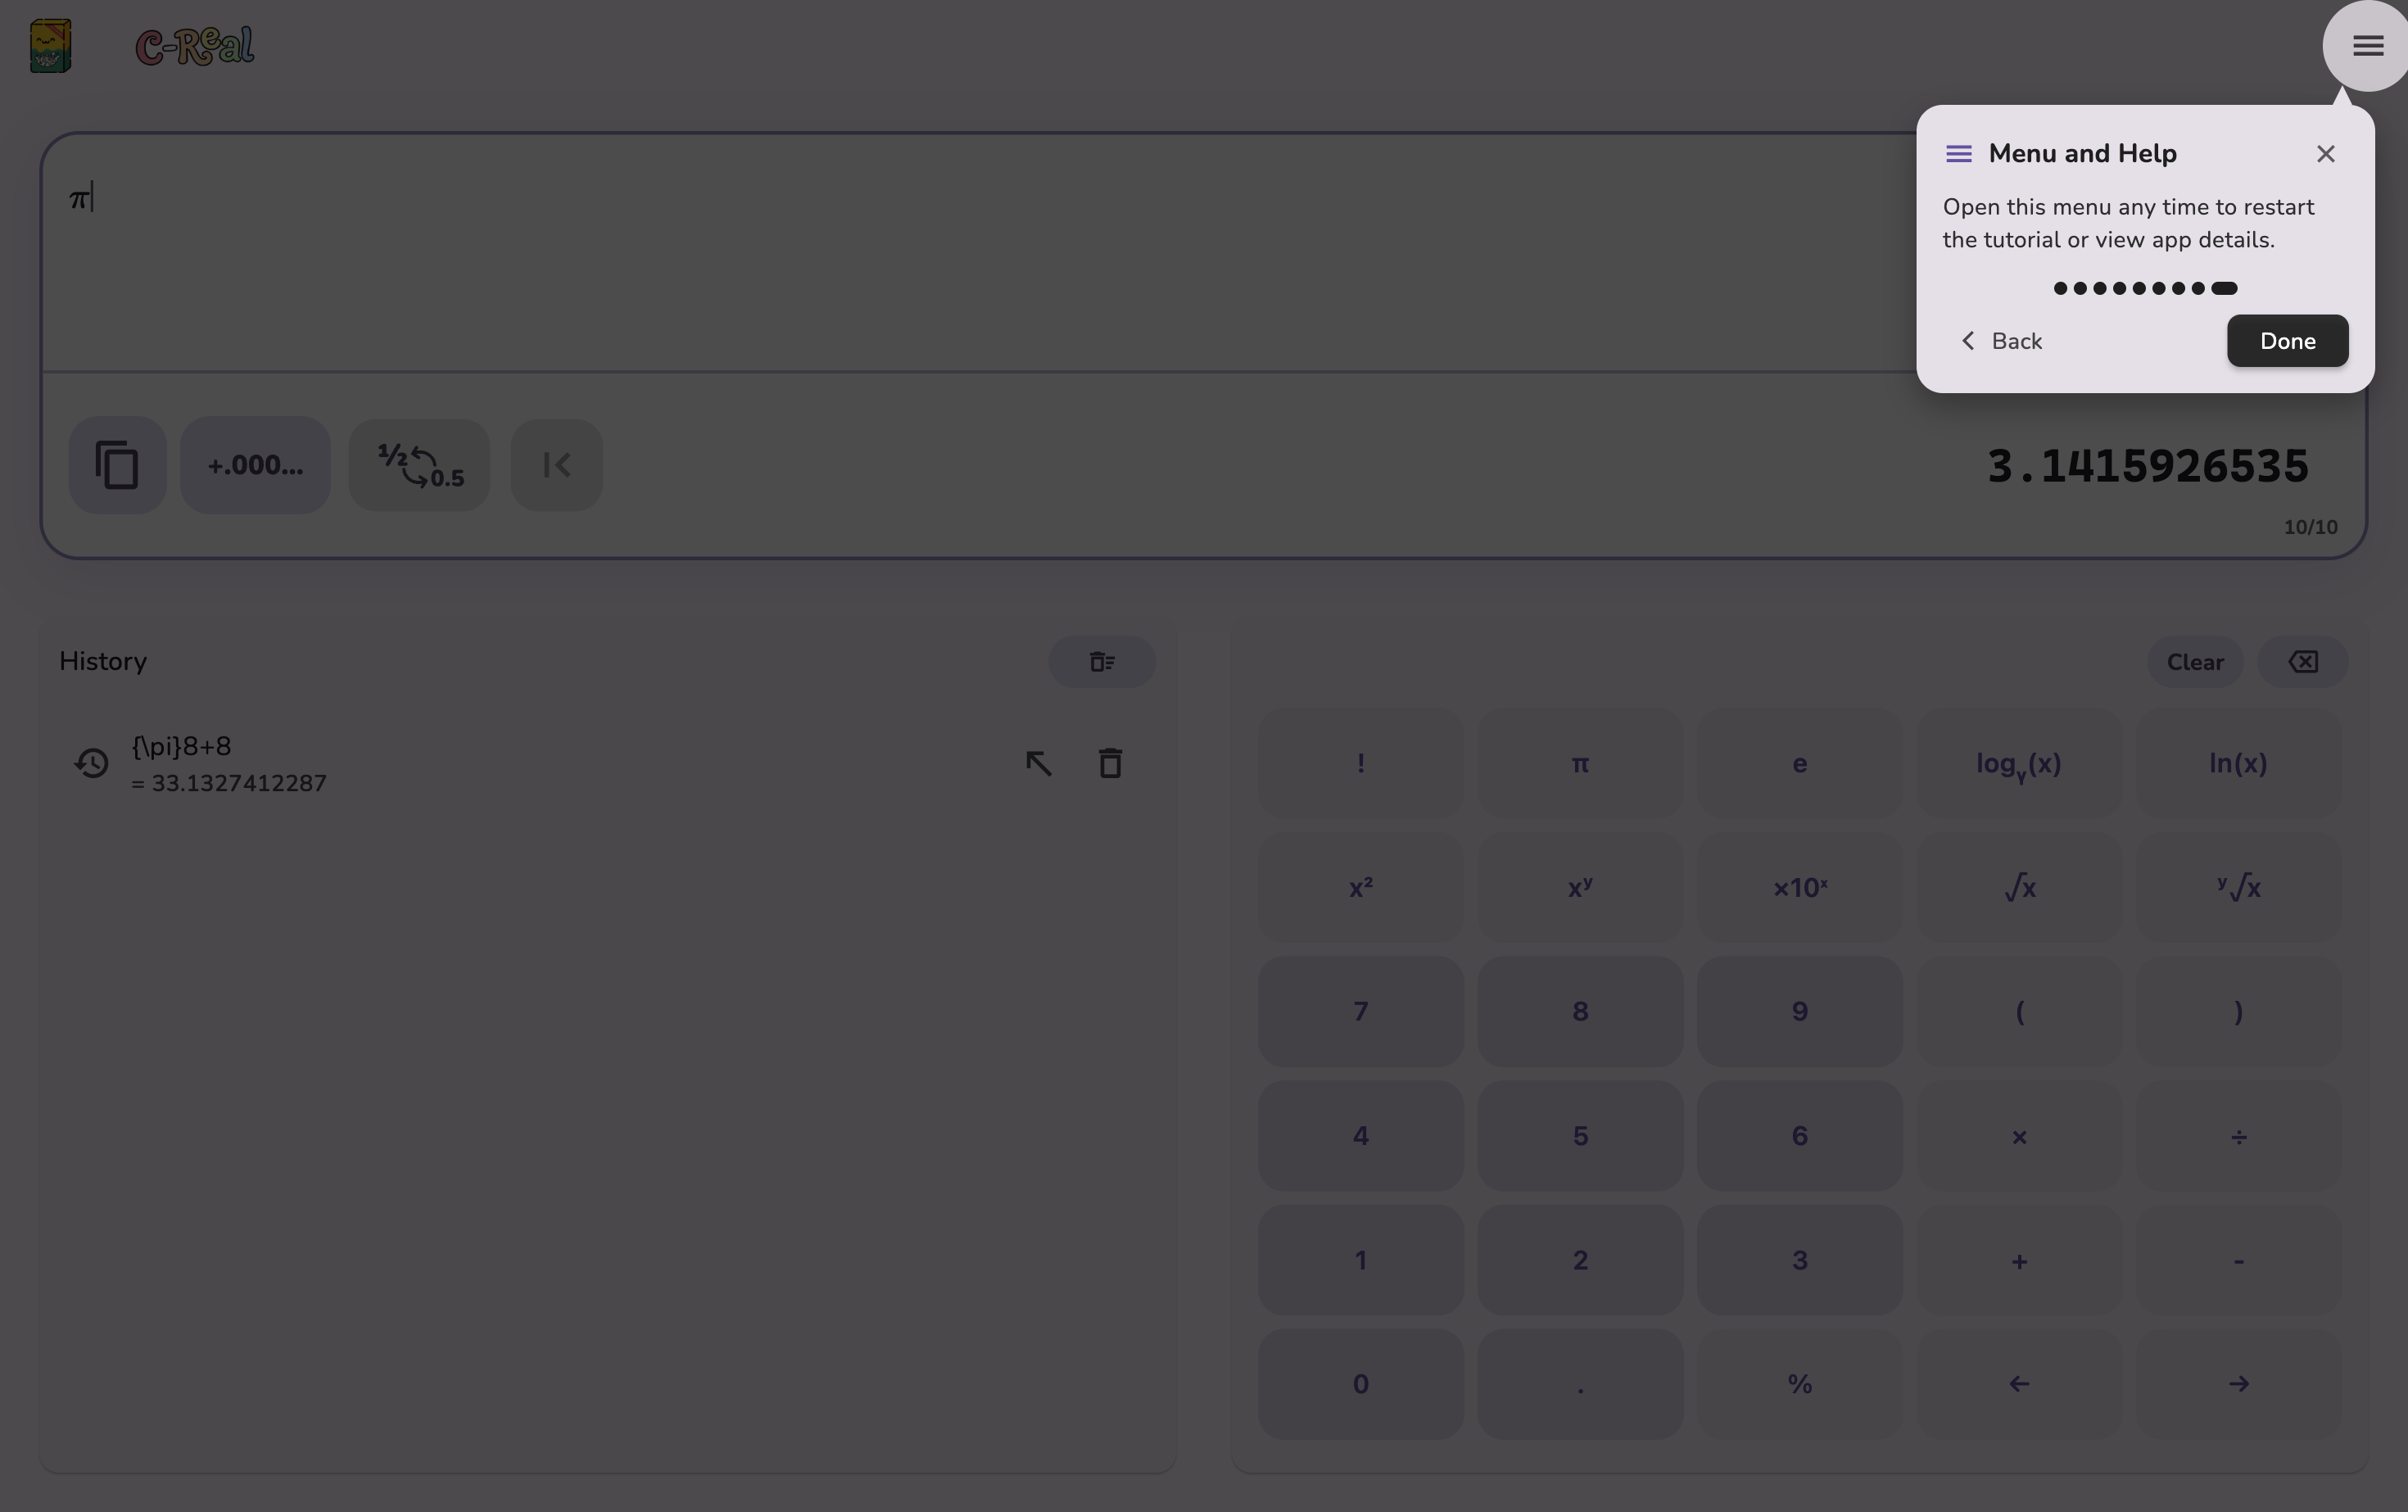
\includegraphics[width=0.6\textwidth]{images/nineth.png}
    \caption{Tlačitko pro informace}
    \label{fig:menu-and-help}
\end{figure}

Tato část aplikace poskytuje přístup k doplňkovým možnostem, jako je opětovné spuštění tutoriálu nebo zobrazení informací o aplikaci. Uživatel se sem může kdykoli vrátit pomocí nabídky v pravém horním rohu.

\clearpage
\newpage

\listoffigures

\end{document}
